\chapter{Introduction}
Video games rely on real-time physics engines to provide realistic environments. This is noticeable in 3D gaming where players expect fast paced interaction. This requirement has produced significant commercial activity resulting in physics engines for real-time simulation for rigid body dynamics. Although realism is convincing, a degree of mathematical accuracy is usually sacrificed (causing error) in order to attain real-time delivery within constrained resource settings. However, with significant commercial effort, the mathematical error has reduced over the years and commercial game engines are finding their use in other industries (e.g.,  \cite{Xu2017, Lu2017, Shah2018}).

Combining physics engines with game engines (e.g., Unity, Unreal), presents a cost-efficient development platform for developing realistic environments. These gaming environments may be presented to geographically distant players using server-side scalable technologies. This allows scalable gaming platforms, presenting players with large online worlds to explore whilst maintaining the visually highly realistic environments generated by the player's local machine. Research into delivering scalability in such online worlds is focused on balancing real-time and consistency issues for enabling player-player interaction. The evolution of such research can be traced back to the earliest work on game area subdivision \cite{Npsnet} through player-focused game area sub-division (e.g., \cite{Morgan2005InterestManagement, Greenhalgh}) and eventually to the many commercial cloud based solutions as described by \cite{iCloudAccess}.

The problem of scalable player-player interaction is not a solved problem, as the numerous interaction possibilities across gaming genres and the latency in networks provides many different possible bespoke solutions. Player interaction can be measured in milliseconds, which current networking technology cannot model for all gaming genres in a scalable manner without giving rise to inconsistency. Therefore, the notion of trying to model real-time physics, which requires solvers working in iterations measured in microseconds, would be considered a near impossible task. However, achieving this would allow the physics engine element of the gaming console to be transplanted to the server-side (cloud), freeing up resources for game-play and rendering on a player's local machine.

Streamed gaming is an active area of research (e.g., \cite{GARCIAVALLS}), where the game is executed on the server-side and the player interacts remotely (e.g., \cite{PSNOW, NVidiaGameStream}). The existence of such services suggests the possibility of real-time interaction for all gaming genres across cloud infrastructures. Therefore, our problem is concentrated on distributing the physics engine element of such technologies across the server-side while maintaining the real-time streamed service to players.

Recent developments have demonstrated the importance of software defined networks (SDN) for presenting timely cloud solutions \cite{Wang, Kumar}. The SDN manages the distribution of messages across servers in the most economical way possible (e.g., resource usage). The fact that SDNs can produce timely messaging across tightly coupled server-side deployments (the cloud) suggests the possibility that timely requirements for scalable physics delivery can be fulfilled.

In the context of current research, we can place ourselves at the juncture of balancing physics calculations across servers in the cloud for game streaming services. This should provide improved economic use of resources, as current game streaming services simply mimic the machine requirements of the player without distributing any of the component parts of the gaming engine. In addition, streamed games may benefit from increased numbers of artefacts (way beyond what is currently possible in a player's machine) as other servers may be utilised to solve the physics problems.

To achieve our research goal while remaining relevant to current state-of-the-art physics simulations, this study uses PhysX (from Nvidia) as the physics engine \cite{PhysX}. This ensures a simulation equal in detail to commercial video game titles. The challenge is to deploy instances of PhysX into a cloud infrastructure (on multiple servers) and allow objects within a simulation to be seamlessly passed across PhysX instances. We construct messaging services to enable PhysX instances on different servers to communicate and divide the simulation geographically across such servers. The challenge of this research is ensuring real-time fidelity can be satisfied when objects migrate across PhysX instances (from server to server). This problem of object migration is complicated by the possibility of object interaction occurring during such migration. Considering the assumption of commercial level fidelities of fast paced objects and frame rates of 60 frames per-second, any anomalous behaviour of objects during migration would be easily discernible to a player. 

\section{Summary}
Scaling and more complex games is a selling point.

Traditionally real-time simulations are confined to a single machine, including real-time physics. 
Recent cloud technology has made available, lower cost, low-latency, high-performance, including GPU-enabled machines. This means, real-time simulations can now run in the cloud as well as being economically viable. It is possible to rapidly provision resources on demand, allowing for fast scaling up and down of resources as needed.

The potential uses of scaling real-time physics simulations are vast. (Large world, physics based games, game relying on physics queries (AI)). Scaling real-time physics is useful not only for games, but large-scale simulations where querying or simulating the physical state of the world is heavily used, e.g. large-scale multi-agent AI, such as city simulations, military simulations. 

Server authoritative physics would also allow over the network multiplayer games to rely heavily on physical elements. In games, only a limited part of the game is simulated on the server side and not physics, with focus on player-player interaction and not player-environment (physics) interaction, as this is a limit of existing technology. 
Synchronising physics states between players and servers is not possible due to latency, two players will have different views of the physical state of the world, based on their latency, interactions from those player's with the physical state will cause divergence, which may not be possible to converge. This is normally worked around by not having physics affect gameplay and using kinematic sequences, ensuring determinism. A single physics simulation, resolves these problems of multiple physics states, which have to be synchronised and lead to divergent physics states. 

Simulating the physical state of the world entirely in the cloud frees up resources on the user's machine allowing for more processing time to be spent on other systems, such as graphics, AI etc. Alternatively, simulating physics in the cloud could be combined with streamed gaming.

Streamed gaming is an active area of research, where the game is run entirely in the cloud, with the graphical output streamed to the player. Reducing the computing power requirements on player hardware even allowing gaming on mobiles with graphical quality beyond what would be possible if the game were running entirely on a mobile device.  If the physics simulation is co-located with the graphics streaming servers (with very low-latency), the problem of latency between player's view of the physics simulation and actual state is resolved, allowing for a better shared view of the physics state.

It therefore is the next logical step to start breaking apart the different systems of the game into their own 'containers', allowing for independent scaling and resource provision management.  
Using the recent developments in cloud technology, we explore the possibility of using this on demand scaling, to scale up real-time physics simulations.


\section{Purpose of Study}
\section{Outline}

\chapter{Background and Related Work}
\section{Real-time Physics Engines}
%We must first understand how real-time physics engines work
%"World" is called a scene, "Bodies" are things being simulated
%Descrete simulation steps, each step simulates a period of time

%Main physics loop (what goes on within a simulation step)
%Explanation of rigid bodies, actors, shapes, constraints
%Explanation of simulation and query shapes
%Explanation of trigger volumes
%Explanation of kinetic vs kinematic
%Explanation of sleeping

%Each simulation step must take less time to execute than the time it is simulating, otherwise the simulation is unable to run in real-time.
%It is possible for the main application to update more often than the simulation frequency
%It is also possible that the main application update is unable to be executed at the same frequency as the physics simulation frequency. Options are running the simulation at a bigger time-step or simulate multiple, smaller sub-steps. Trade-off between keeping consistent behaviour and performance.
%Diagrams for above
%Well of despair example and diagram
%Solutions to well of despair: 
%Decouple physics from application update with use of sync and async scene, can make player interaction more difficult
%allow time dropping
%variable time-stepping
%simplifying the physics scene

%PhysX runs on a separate thread by default
%It is not possible to read/write directly to the scene during simulation, scene is buffered so changes can be made and will only affect the next simulation step. 
%Image of time-slots
%Event callbacks for collisions/triggers

\section{Online Gaming}
Although there has been research utilising multiple servers to distribute the task of solving physics based problems (e.g., \cite{mashayekhi2018automatically}), to the best of our knowledge there is no literature describing real-time interactive physics exploiting the addition of servers to gain scalability. The closest work to our research is that carried out to seek scalability in terms of player numbers in online gaming in the field of Distributed Virtual Environments (DVEs). 

There are primarily two ways in which server-side resources can provide scalability in online gaming (e.g., DVEs): (1) Migratory; (2) Non-migratory. In migratory approaches, a server will assume responsibility for handling in-simulation objects within a region. When objects traverse region boundaries into a region that is the responsibility of another server, they will be handed over to the other server. In a non-migratory approach, in-simulation objects are allocated to the responsibility of a particular server at instantiation time and stay with that server until they are deleted.

The benefit of a migratory approach is that tightly coupled objects (interacting frequently) can be co-located on the same server, reducing interaction latencies. However, the act of moving such objects may be costly in terms of time required to resolve the hosting requirements of an object. The benefit of a non-migratory approach is that servers are rarely exhausted but network traffic will result in higher latencies that will inhibit the fidelity of interaction between objects.

Migratory and non-migratory approaches are now described in greater detail.

\section{Distributed Virtual Environments}
 In the migratory approach, a single game world exists, but is divided into geographical regions. Each region is maintained by a separate server (e.g. \cite{AnOverlappingArchitecture, ScalabilityIssues, LoadBalancingForDistributedVR, ALoadBalancingAlgorithm, SpatialOS}). The main drawback of this approach is the complexity of handling interactions between objects in different regions/servers while maintaining consistency \cite{P2PForMMOs}. A technique to minimise these issues is to use overlapping regions between spatial partitions. Servers share state information about objects in the overlapping region (examples include 'zoning' as described in \cite{AnOverlappingArchitecture} or 'sub-regions' as described in \cite{ScalabilityIssues}). Examples of games using this technology include \cite{Vanishin30:online} and \cite{WorldsAd48:online}, which use the SpatialOS platform \cite{SpatialOS}. However, the techniques used by SpatialOS are not described in any literature. Their demonstration video exhibits unnatural object "jitter", which is possibly a result of network latency. 
 
In the non-migratory approach, the game world is not divided into geographical regions and players are split between servers in one of two ways: (1) Several instances of the game world run with complete independence from one another (known as shards e.g.\cite{WOW}) and players have no interaction across shards \cite{P2PForMMOs}; (2) Players are distributed amongst servers by some other non-geographical method and interactions with players on other servers requiring servers to share messages \cite{LoadBalancingforMMOs}.

Although shards allow a degree of scalability in the number of players, it is not suitable for use in scaling real-time physics simulations as all entities within a real-time physics simulation, in the same geographical region, may interact with each other.

In the case of architectures not using shards, Interest Management is required to prevent message passing growing polynomially as players increase (e.g. \cite{Bezerra2008} and \cite{LoadBalancingforMMOs}).
\cite{Bezerra2008} proposes the A3 algorithm, an interest management technique for distributed simulations aiming to significantly reduce the necessary bandwidth required between servers. A3 uses a combination of a circular area of interest and field of view combined with a relevance gradient. \cite{LoadBalancingforMMOs} proposes a Behavioural Interest Management Technique that allocates resources based on player interactions. Auras (an area of interest/influence) are used to determine player message exchanges, reducing message passing while promoting player number scalability.

Despite DVE being a popular area of research, the literature is restricted to modelling player interaction across servers and balancing their support on different servers. Clearly, the interaction patterns of players are significantly less demanding in terms of timeliness than that of interacting physical objects.

\section{Streamed Gaming}
Streamed Gaming (also know as Gaming as a Service) consists of cloud servers streaming to a player's device with player input being returned to the cloud server. The player's device acts as a thin client. The main benefit is that a player does not require expensive, powerful hardware, and games can be played on any operating system (e.g. Android, Linux and Mac). However, these benefits come at the cost of bandwidth and latency requirements \cite{iCloudAccess}.

Streamed Gaming services currently available include \cite{NVidiaGameStream} and \cite{PSNOW}. NVIDIA GRID technology is targeted specifically at Streamed Gaming \cite{NVIDIACloud}.

A drawback to streamed gaming is the requirement for a significantly more powerful machine at the server-side than what would be required if the game was played solely at the client side. This is because the server not only has to run the game, but has to process the video and audio stream into a suitable format for streaming. In addition, real-time player interaction requires low latency and high bandwidth resulting in networking infrastructure more expensive than would be expected for regular streaming services. 

In streamed gaming, each game instance resides on a single server. There is no technology to balance the real-time requirements of the game across multiple servers. The core problem is that all gaming technology is built and designed for single console/PC install and the greatest bottleneck is the inability to share physics calculations across machines.

\section{Cloud Computing}
Previously scaling up software would require a single machine with more computing power or a dedicated cluster. Cloud computing allows for on demand allocation of resources, dramatically cutting the cost. There has been a big move to abstract architecture away from the applications running on it, containers such as docker and even further with things like Google's App Engine.

\section{Scalable Non-Real Time Physics}
Includes fluid simulations, meteorological simulations. Non-real time physics simulation work very differently from real-time, accuracy is highly favoured as opposed to the fast, plausible simulations in real-time physics. In addition high latency (10s of ms) is a small issue relative to large time-steps.

\section{Background Summary}
In physics simulations, there must be an object present in the solving phase for it to be considered in the overall solution of the scenario. A non-migratory approach requires a "ghost" representation of the object in a remote server to enable interaction. Given the calculations and discretisation steps, a "ghost" object takes up just as many resources in deriving a solution as a real object. This rules out the non-migratory approach for our problem. This leaves migratory.

Migratory approaches are concerned with managing the network traffic for those entities that could possibly exist on two servers but can only be solved on one. Such objects need to be placed with an owning server while minimising the effect of thrashing (where an algorithm frequently transfers objects between servers). In the rest of this paper, we describe our approach to solving this algorithmically, present how a working implementation was achieved, and present results evidencing our work. This is the first presentation of literature that can demonstrate real-time scalable server-side physics modelling and is a significant contribution to reducing the cost of commercialised streamed gaming.

\chapter{Problem Definition and Proposed Solution}
Our approach allows servers to assume responsibility for objects within a real-time simulation without hindering the fidelity of such a simulation. In order to maintain scalability, the extra processing overhead must be less than that gained by distributing the simulation workload. 
	
\definecolor{wrwrwr}{rgb}{0.3803921568627451,0.3803921568627451,0.3803921568627451}
\definecolor{dtsfsf}{rgb}{0.8274509803921568,0.1843137254901961,0.1843137254901961}
\definecolor{sexdts}{rgb}{0.1803921568627451,0.49019607843137253,0.19607843137254902}
\definecolor{rvwvcq}{rgb}{0.08235294117647059,0.396078431372549,0.7529411764705882}
\begin{figure}
	\centering
	\begin{tikzpicture}[line cap=round,line join=round,>=triangle 45,x=1cm,y=1cm, scale=2.4]
	%	\clip(-3.8316065591348587,-1.5915496679322039) rectangle (4.0193993686026035,3.119053888710274);
	\draw [line width=2pt,color=sexdts,fill=sexdts,fill opacity=0.6] (0.11306222137602934,0.5749956216017253) circle (0.2191629059122392cm);
	\fill[line width=2pt,color=dtsfsf,fill=dtsfsf,fill opacity=0.6] (-0.19130495931412153,2.497904290969918) -- (0.09727089010996666,2.49668178609732) -- (0.09849339498256493,2.785257635521408) -- (-0.19008245444152327,2.7864801403940063) -- cycle;
	\draw [line width=2pt,color=sexdts,fill=sexdts,fill opacity=0.6] (0.2690682445566622,2.8641372386638633) circle (0.18190589696740675cm);
	\fill[line width=2pt,color=dtsfsf,fill=dtsfsf,fill opacity=0.6] (-0.18001743348774918,1.688638597893834) -- (0.12779907363732385,1.6894047421549492) -- (0.12703292937620878,1.997221249280022) -- (-0.1807835777488642,1.996455105018907) -- cycle;
	\draw [line width=2pt,color=sexdts,fill=sexdts,fill opacity=0.6] (0.3506985149669561,2.1504628052606924) circle (0.20094089799255885cm);
	\fill[line width=2pt,color=rvwvcq,fill=rvwvcq,fill opacity=0.65] (-0.336221735744061,-0.21399083968233576) -- (-0.08697438199196733,-0.21915612145269675) -- (-0.08966346659279195,0.37774900628071006) -- (-0.336221735744061,0.37774900628071006) -- cycle;
	\draw [line width=2pt,color=dtsfsf,fill=dtsfsf,fill opacity=0.6] (-2.7581115521258512,-0.5210040634712074) circle (0.18765298545020567cm);
	\draw [line width=2pt,color=dtsfsf,fill=dtsfsf,fill opacity=0.6] (-2.4332540697970817,-0.7399608687412594) circle (0.1836317971285386cm);
	\draw [line width=2pt,color=dtsfsf,fill=dtsfsf,fill opacity=0.6] (-2.7438006498206193,-0.983246207930206) circle (0.20084779094096714cm);
	\fill[line width=2pt,color=dtsfsf,fill=dtsfsf,fill opacity=0.6] (-1.8,-0.3) -- (-1.5507526462479064,-0.30516528177036095) -- (-1.553441730848731,0.29173984596304586) -- (-1.8,0.29173984596304586) -- cycle;
	\draw [line width=2pt,color=dtsfsf,fill=dtsfsf,fill opacity=0.6] (-1.519067473250276,-0.8075899850392314) circle (0.2110032461078136cm);
	\draw [line width=2pt,color=dtsfsf,fill=dtsfsf,fill opacity=0.6] (-1.3242760580159627,-0.35254200026346094) circle (0.220457331048815cm);
	\fill[line width=2pt,color=rvwvcq,fill=rvwvcq,fill opacity=0.6] (1.6172164649279959,-0.10848935040022167) -- (1.9441305251416572,-0.10779885294426608) -- (1.9434400276857018,0.21911520726939515) -- (1.6165259674720405,0.21842470981343975) -- cycle;
	\draw [line width=2pt,color=sexdts,fill=sexdts,fill opacity=0.6] (2.1773098805776194,-0.021729373301184463) circle (0.19660778801195347cm);
	\fill[line width=2pt,color=sexdts,fill=sexdts,fill opacity=0.6] (2.3730665457464766,-0.11747262438789227) -- (2.7159883030391594,-0.11287162500071371) -- (2.7113873036519816,0.23005013229196902) -- (2.3684655463592983,0.2254491329047909) -- cycle;
	
	% Boundary Lines
	\draw [line width=1pt, dash pattern=on 5pt off 5pt] (-3,0)-- (0,0);
	\draw [line width=1pt, dash pattern={on 4pt off 3pt on 1pt off 3pt}] (0,3)-- (0,0);
	\draw [line width=1pt, dash pattern={on 2pt off 2pt}] (0,0)-- (3,0);
	
	% Server Labels
	\draw (-1.5,3.5) node[anchor=center] {Server 0};
	\draw (1.5,3.5) node[anchor=center] {Server 1};
	\draw (0,-1.0) node[anchor=center] {Server 2};
	
	\draw [line width=2pt,dash pattern=on 1pt off 1pt] (0.11306222137602934,0.5749956216017253) circle (0.33970250416397074cm);
	\draw [line width=2pt,dash pattern=on 1pt off 1pt] (0,1.824163562143371) circle (0.3724807823065095cm);
	\draw [line width=2pt,color=dtsfsf] (-0.19130495931412153,2.497904290969918)-- (0.09727089010996666,2.49668178609732);
	\draw [line width=2pt,color=dtsfsf] (0.09727089010996666,2.49668178609732)-- (0.09849339498256493,2.785257635521408);
	\draw [line width=2pt,color=dtsfsf] (0.09849339498256493,2.785257635521408)-- (-0.19008245444152327,2.7864801403940063);
	\draw [line width=2pt,color=dtsfsf] (-0.19008245444152327,2.7864801403940063)-- (-0.19130495931412153,2.497904290969918);
	\draw [line width=2pt,color=dtsfsf] (-0.18001743348774918,1.688638597893834)-- (0.12779907363732385,1.6894047421549492);
	\draw [line width=2pt,color=dtsfsf] (0.12779907363732385,1.6894047421549492)-- (0.12703292937620878,1.997221249280022);
	\draw [line width=2pt,color=dtsfsf] (0.12703292937620878,1.997221249280022)-- (-0.1807835777488642,1.996455105018907);
	\draw [line width=2pt,color=dtsfsf] (-0.1807835777488642,1.996455105018907)-- (-0.18001743348774918,1.688638597893834);
	\draw [line width=2pt,color=rvwvcq] (-0.336221735744061,-0.21399083968233576)-- (-0.08697438199196733,-0.21915612145269675);
	\draw [line width=2pt,color=rvwvcq] (-0.08697438199196733,-0.21915612145269675)-- (-0.08966346659279195,0.37774900628071006);
	\draw [line width=2pt,color=rvwvcq] (-0.08966346659279195,0.37774900628071006)-- (-0.336221735744061,0.37774900628071006);
	\draw [line width=2pt,color=rvwvcq] (-0.336221735744061,0.37774900628071006)-- (-0.336221735744061,-0.21399083968233576);
	\draw [line width=2pt,dash pattern=on 1pt off 1pt] (-0.20008010870040147,0.05759193325942933) circle (0.4395227390987423cm);
	\draw [line width=2pt,dash pattern=on 1pt off 1pt] (-2.7581115521258512,-0.5210040634712074) circle (0.3403858079791503cm);
	\draw [line width=2pt,dash pattern=on 1pt off 1pt] (-2.4332540697970817,-0.7399608687412594) circle (0.3064438391841357cm);
	\draw [line width=2pt,dash pattern=on 1pt off 1pt] (-2.7438006498206193,-0.983246207930206) circle (0.32740392092189946cm);
	\draw [line width=2pt,color=dtsfsf] (-1.8,-0.3)-- (-1.5507526462479064,-0.30516528177036095);
	\draw [line width=2pt,color=dtsfsf] (-1.5507526462479064,-0.30516528177036095)-- (-1.553441730848731,0.29173984596304586);
	\draw [line width=2pt,color=dtsfsf] (-1.553441730848731,0.29173984596304586)-- (-1.8,0.29173984596304586);
	\draw [line width=2pt,color=dtsfsf] (-1.8,0.29173984596304586)-- (-1.8,-0.3);
	\draw [line width=2pt,dash pattern=on 1pt off 1pt] (-1.6811522710982656,0.015633897433233776) circle (0.4555571106906273cm);
	\draw [line width=2pt,dash pattern=on 1pt off 1pt] (-1.519067473250276,-0.8075899850392314) circle (0.40351234312900314cm);
	\draw [line width=2pt,dash pattern=on 1pt off 1pt] (-1.3242760580159627,-0.35254200026346094) circle (0.3214616358035378cm);
	\draw [line width=2pt,color=rvwvcq] (1.6172164649279959,-0.10848935040022167)-- (1.9441305251416572,-0.10779885294426608);
	\draw [line width=2pt,color=rvwvcq] (1.9441305251416572,-0.10779885294426608)-- (1.9434400276857018,0.21911520726939515);
	\draw [line width=2pt,color=rvwvcq] (1.9434400276857018,0.21911520726939515)-- (1.6165259674720405,0.21842470981343975);
	\draw [line width=2pt,color=rvwvcq] (1.6165259674720405,0.21842470981343975)-- (1.6172164649279959,-0.10848935040022167);
	\draw [line width=2pt,color=sexdts] (2.3730665457464766,-0.11747262438789227)-- (2.7159883030391594,-0.11287162500071371);
	\draw [line width=2pt,color=sexdts] (2.7159883030391594,-0.11287162500071371)-- (2.7113873036519816,0.23005013229196902);
	\draw [line width=2pt,color=sexdts] (2.7113873036519816,0.23005013229196902)-- (2.3684655463592983,0.2254491329047909);
	\draw [line width=2pt,color=sexdts] (2.3684655463592983,0.2254491329047909)-- (2.3730665457464766,-0.11747262438789227);
	\draw [line width=2pt,dash pattern=on 1pt off 1pt] (1.7707737818301332,0.042356814063601776) circle (0.3324655775151698cm);
	\draw [line width=2pt,dash pattern=on 1pt off 1pt] (2.5485828739333973,0.0529545076040507) circle (0.31587509276975684cm);
	
	% Object labels
	\draw[color=dtsfsf] (-0.5,3) node {A};
	\draw[color=sexdts] (0.75,3) node {B};
	\draw[color=dtsfsf] (-0.6,1.9) node {C};
	\draw[color=sexdts] (.75,1.9) node {D};
	\draw[color=dtsfsf] (-1.66,0.75) node {E};
	\draw[color=dtsfsf] (-0.85,-0.35) node {F};
	\draw[color=dtsfsf] (-1.5,-1.45) node {G};
	\draw[color=dtsfsf] (-3.3,-0.5) node {H};
	\draw[color=dtsfsf] (-2.2,-1.2) node {I};
	\draw[color=dtsfsf] (-3.3,-1) node {J};
	\draw[color=sexdts] (2.2,-0.5) node {K};
	\draw[color=sexdts] (2.5,0.5) node {L};
	\draw[color=rvwvcq] (1.8,-0.5) node {M};
	\draw[color=rvwvcq] (-0.6,0.6) node {N};
	\draw[color=sexdts] (0.5,1) node {O};
	
	\end{tikzpicture}
	
	\begin{tikzpicture}[line cap=round,line join=round,>=triangle 45,x=1cm,y=1cm, scale=0.75, every node/.style={font=\scriptsize,
		minimum height=0.25cm,minimum width=0.5cm},scale=0.75]
	\clip(-8,-0.05) rectangle (4,2.15);
	
	% Boundary Lines
	\draw [line width=1pt, dash pattern={on 4pt off 3pt on 1pt off 3pt}] (-7.5,1.8)-- (-6.5,1.8);
	\draw (-6,1.8) node[anchor=west] {0-1 Boundary};
	\draw [line width=1pt, dash pattern=on 5pt off 5pt] (-7.5,1.3)-- (-6.5,1.3);
	\draw (-6,1.3) node[anchor=west] {0-2 Boundary};
	\draw [line width=1pt, dash pattern={on 2pt off 2pt}] (-7.5,0.8)-- (-6.5,0.8);
	\draw (-6,0.8) node[anchor=west] {1-2 Boundary};
	
	\draw [line width=2pt] (-7.5,0.3)-- (-6.5,0.3);
	\draw (-6,0.3) node[anchor=west] {Aura};
	
	% Object boxes
	\fill[line width=2pt,color=sexdts,fill=sexdts,fill opacity=0.6] (0.2,0.8) -- (0.7,0.8) -- (0.7,1.3) -- (0.2,1.3) -- cycle;
	\fill[line width=2pt,color=rvwvcq,fill=rvwvcq,fill opacity=0.6] (0.2,-0.0) -- (0.7,-0.0) -- (0.7,0.5) -- (0.2,0.5) -- cycle;
	\fill[line width=2pt,color=dtsfsf,fill=dtsfsf,fill opacity=0.6] (0.2,1.6) -- (0.7,1.6) -- (0.7,2.1) -- (0.2,2.1) -- cycle;
	
	\draw [line width=2pt,color=sexdts] (0.2,0.8)-- (0.7,0.8);
	\draw [line width=2pt,color=sexdts] (0.7,0.8)-- (0.7,1.3);
	\draw [line width=2pt,color=sexdts] (0.7,1.3)-- (0.2,1.3);
	\draw [line width=2pt,color=sexdts] (0.2,1.3)-- (0.2,0.8);
	
	\draw [line width=2pt,color=rvwvcq] (0.2,-0.0)-- (0.7,-0.0);
	\draw [line width=2pt,color=rvwvcq] (0.7,-0.0)-- (0.7,0.5);
	\draw [line width=2pt,color=rvwvcq] (0.7,0.5)-- (0.2,0.5);
	\draw [line width=2pt,color=rvwvcq] (0.2,0.5)-- (0.2,-0.0);
	
	\draw [line width=2pt,color=dtsfsf] (0.2,1.6)-- (0.7,1.6);
	\draw [line width=2pt,color=dtsfsf] (0.7,1.6)-- (0.7,2.1);
	\draw [line width=2pt,color=dtsfsf] (0.7,2.1)-- (0.2,2.1);
	\draw [line width=2pt,color=dtsfsf] (0.2,2.1)-- (0.2,1.6);
	
	\draw (1.0,2.2) node[anchor=north west] {Server 0 Object};
	\draw (1.0,1.4) node[anchor=north west] {Server 1 Object};
	\draw (1.0,0.6) node[anchor=north west] {Server 2 Object};
	
	\end{tikzpicture}
	\caption{Aura Projection Scenarios}
	\label{AuraProj}
\end{figure}

\section{Naive Approach}\label{CrossBoundaryInteraction}
To provide a comparison and to demonstrate our contribution to the field, a naive approach is described first. The naive approach is used to highlight the challenges faced when solving this problem.

Assuming a migratory approach in which servers are responsible for a geographic area, when one object crosses a boundary between geographic areas, such an object's hosting must be transferred to the appropriate server. It is handling this transfer that is the underlying problem.

Accomplishing a transfer with a simple message from one server to another is charged with many problems: (1) the message may be lost and the object disappears; (2) the message may be delayed and the object disappears and reappears; (3) there may be more than one candidate server for hosting (if object travelling quickly) resulting in duplication of an object; (4) the server an object leaves may be unaware of when it should stop simulating the object (resulting in duplicated objects)\cite{High-performanceServerSystems}; (5) an object may be colliding with another object across the boundary which would be lost if both objects are hosted on different servers (objects may pass through each other).

For additional clarity consider objects A and B in Fig. \ref{AuraProj}. Each server is aware of the objects they host but not other objects. As such, objects A and B would not interact and not collide with each other, creating a time-space inconsistency. A time-space inconsistency is defined as two objects occupying the same space at the same time. If Object B has a velocity directed towards the boundary, it would continue at its initial velocity until it traversed the boundary, at which point it would migrate to server 0. Upon completion of the migration, objects A and B would overlap far more than would be expected in a typical simulation, resulting in inappropriate collision response.

\section{Considered Solutions}
There are several solutions that should be considered to distribute a real-time physics simulation across multiple machines over a network:

\subsection{Both servers simulate objects on boundary}
Simulate objects overlapping the boundary on both servers, however, results would diverge significantly as objects interact with objects not overlapping the boundary and there is the extra computational overhead of needing to be simulate objects twice.

\subsection{Both servers simulate objects in an overlapping region}
Simulate objects overlapping the boundary and objects interacting with those on both servers, e.g. by using an overlapping region. Object may interact with objects not in the overlapping region, so the results would diverge or the overlapping region would have to dynamically change in order to keep all interacting objects within the overlapping region. Even if all objects interacting were in the overlapping region, results would still diverge due to non-determinism of physics engines. The divergence of results due to non-determinism could be corrected by periodically syncing the objects (ensuring the objects have the same state on both servers), however, this would appear as jitter and would require additional computational and network overhead. In addition to this there is the extra computational overhead of needing to be simulate objects twice.

\subsection{Over network object collisions}
Objects in the overlapping region interact over the network. This could be done synchronously, which would be slow (could divide collision responses between servers and then exchange results). This solution would have to simulate objects twice and would require multiple round-trips of messages over the network per physics time-step, but the collision response for objects would be identical on both servers.

% All these solutions require fast and reliable network connections, except AP

\subsection{Remote objects as static}
Treat objects being simulated on another server as static. However, this would not lead to correct collision response, if compared to a single simulation. Momentum is conserved in collisions and no momentum is transferred to static objects, therefore the resulting momentum on the colliding object would not be the same as if the two objects were dynamic (not static) on a single simulation.
Half of all collisions would be missed, as collisions would be resolved for the object not being treated as static, but on the remote server, the collision never appears to happen, as the collision has already been resolved when receiving the updated state of the interacting object.
This could also lead to jitter, if two objects are in contact (i.e. colliding over multiple frames, such as a box stacked on top of another box), the server in which the collision is resolved on could be different every physics step, the outcome of which may be different and cause jitter.
% It is probably more complicated than this, as physics engines do a lot to deal with objects in contact, constantly moving a static object is probably going to interfere with this.

% Collisions may not be missed if there is deep penetration as PhysX won't move objects all the way out of a collision if the collision is deep enough.

\subsection{All object interactions on same server}
Simulate all objects that are interacting with each other on the same server. Auras could be used to determine which objects are potentially interacting. Auras of objects would need to be exchanged. Solution would need to manage number of auras exchanged to reduce this overhead.

\section{Proposed Solution}
% Introduce this in context of above section
We term our approach Aura Projection (AP). AP tackles the problem of maintaining consistency across regions while ensuring timeliness of a simulation. In particular, AP provides the building blocks of a scalable solution to server-side physics simulations by handling all configurations of boundary cases in migratory approaches. 

In AP, an object maintains an aura, an area of interest around the object, that indicates its possible future location and, therefore, aids in identifying near future interactions. In other words, auras act as a request for objects to be migrated. Any object colliding with the aura is migrated to the server the aura came from. The presence of an aura allows: (1) the prediction of future hosting requirements allowing time to transfer objects; (2) a narrowing of interest in only considering a subset of objects promoting a scalable solution; (3) an unhindered physics simulation for existing objects; (4) limiting communications requirements between servers based on focusing message passing overhead on interacting objects (promoting scalability). In essence, AP ensures that any two objects that may be interacting are always being simulated on the same server. For example, objects C and D illustrated in Fig. \ref{AuraProj}. Object C projects its aura into Server 1, Object D collides with the aura and is migrated to Server 0, allowing continued interaction to occur.

Messages are sent between servers where aura overlap occurs across a geographic boundary. We term this phase of the algorithm as an object projecting its aura onto another server. %The receiving server can then predict and prepare for the possibility of interaction if an object was migrated to it. 

In the context of real-time physics simulations, auras appear on the receiving server as a trigger volume (non-physically interacting volume). For each simulation step that an object is projecting an aura, the object's position and calculated aura are sent. As a network optimisation, if the boundary object is not moving, no details are sent and the aura on at a receiving server is unaltered.

When an aura is no longer being projected for an object (boundary not overlapped), the server simulating that object sends a message to any servers receiving the aura to remove the aura of that object.

\section{Aura Calculation}
Calculating an aura size is key to creating a scalable solution balanced against consistency: (1) Auras that are too small will result in a faster simulation but with more missed interactions; (2) Auras that are too large will include more calculations that are simply not required, increasing server load and decreasing scalability. Therefore, how auras are calculated will be carefully described and justified. 

Spheres are used to represent auras. This bounding volume is computationally efficient as rotational calculations are not required in determining its correct alignment. Auras accommodate the displacement of objects using an estimated network latency based on historic monitoring, in addition to the distance a remote object may be predicted to penetrate an aura (considering velocities).

Rather than every object maintaining an aura, which would add overhead to the physics simulation, when an aura is exchanged it accounts for a potential remote object's aura. When an object comes into the aura distance of the region boundary, an aura is created for the object and the aura starts being broadcast to neighbouring servers.

Fig. \ref{sequence_diagram} demonstrates the sequence of events involved when an aura is sent, received, and collided with, resulting in an object migration.

To lower inconsistencies during migration, the following user-defined tolerances are used for the aura calculations: maximum speed; maximum latency time; maximum frame-time. If velocities, latencies, or frame-time are above these tolerances, then stability is no longer guaranteed. This enables AP to deterministically indicate to the overall simulation when latency may be influencing the mutually consistent views of the servers, which in turn manifests as errors in the physics.

To calculate the radius of an aura, the maximum distances travelled by objects within the delay time between simulations must first be calculated. To calculate the maximum distance an object may travel for a given time, the following formula is used: $\triangle s=v\cdot \triangle t$, where $ \triangle s$ is distance, $v$ is speed, and $ \triangle t$ is time. In this context, $ \triangle v$ is substituted with maximum speed tolerance, and $ \triangle t$ will be a multiple of the physics step time (to accommodate discrete time step calculations in the physics engine). $ \triangle t$ can be calculated using the maximum frame-time and maximum latency tolerance, discussed below.

There is a time delay between the aura being created on a host and being created on a receiving server, which is made up of: up to one frame before sending the aura creation message; inter-server latency; up to one frame from the message being received and acted upon; the time delay between the aura being created and the detection of the collision between a potential remote object and the aura by the physics update step. This last time delay is accounted for by rounding the previous delays up to the nearest physics time step.

Using the time delays mentioned above and substituting the relevant tolerances, the maximum displacement time ($Max_{DT}$) of a remote object is calculated using the following equation:
\DeclarePairedDelimiter\ceil{\lceil}{\rceil}
\begin{equation}
T_{R}=\ceil*{\frac{2\cdot T_{F} + T_{L}}{T_{P}}}T_{P}
\end{equation}

$T_{R}$ is the $Max_{DT}$ of a remote object, $T_{F}$ is the frame-time tolerance, $T_{L}$ is the latency tolerance and $T_{P}$ is the physics step time.

The aura has to account for the maximum displacement of both the object on the host server and a potential object on the remote server. The total $Max_{DT}$ will be the sum of: a) the $Max_{DT}$ of a remote object, subtracting one physics time step, as the aura only needs to account for the displacement of the host object after the creation of the aura; b) The following time delays: a time delay of up to one frame time between the physics step of the remote server and the remote server update loop sending the migration message from the migration buffer; a time delay of the latency between servers; a time delay of up to one frame time between the message being received by a host and a host acting on the migration message and creating the migrated object in the physics engine; a delay between the migrated object being created and the collision being detected by the physics update step. This last time delay is accounted for by rounding the previous delays up to the nearest physics time step.

The $Max_{DT}$ of the object on the host that is projecting the aura is therefore calculated using the following equation:
\begin{equation}
T_{H}=T_{R}-T_{P}+\ceil*{\frac{2\cdot T_{F} + T_{L}}{T_{P}}}T_{P}
\end{equation}
$T_{H}$ is the $Max_{DT}$ of the object on the host.

The total $Max_{DT}$ is therefore $T_{R}+T_{H}$, which can be simplified to the following equation:
\begin{equation}
T_{T}=(3\ceil*{\frac{2\cdot T_{F} + T_{L}}{T_{P}}}-1)T_{P}
\end{equation}
$T_{T}$ is the total $Max_{DT}$.

The aura of an object can then be calculated using the following equation: 
\begin{equation}
R_{a}=R_{o}+(V_{t}\cdot T_{T})
\end{equation}
$R_{a}$ is the radius of the aura in $m$, $R_{o}$ is the bounding sphere of the object, $V_{t}$ is the speed tolerance in $m\mathord{\cdot}s^{-1}$ and $T_{T}$ is the total $Max_{DT}$ in $s$.

\begin{figure}[!t]	
	\begin{tikzpicture}[line cap=round,line join=round,>=triangle 45,x=1cm,y=1cm,every node/.style={font=\scriptsize,
		minimum height=0.25cm,minimum width=0.5cm},,scale=1.0]

\draw [line width=1pt,dash pattern=on 5pt off 5pt] (-2.0,6)-- (-2.0,-7.25);
\draw [line width=1pt,dash pattern=on 5pt off 5pt] (2.0,6)-- (2.0,-7.25);
\draw [line width=1pt,dash pattern=on 5pt off 5pt] (6.0,6.0)-- (6.0,-7.25);
\draw [line width=1pt,dash pattern=on 5pt off 5pt] (-6.0,6)-- (-6.0,-7.25);
\draw [->,line width=1pt] (-5.5,4) -- (-2.0,4);
\draw [->,line width=1pt] (-1.5,2.5) -- (2.0,1.5);
\draw [->,line width=1pt] (2.5,0) -- (6.0,0);
\draw [->,line width=1pt] (5.5,-1.5) -- (2.0,-1.5);
\draw [->,line width=1pt] (1.5,-3) -- (-2.0,-4);
\draw [->,line width=1pt] (-2.5,-5.5) -- (-6.0,-5.5);
\fill[line width=2pt,color=blue!20] (-6.5,5) -- (-6.5,4) -- (-5.5,4) -- (-5.5,5) -- cycle;
\fill[line width=2pt,color=blue!20] (-2.5,3.5) -- (-2.5,2.5) -- (-1.5,2.5) -- (-1.5,3.5) -- cycle;
\fill[line width=2pt,color=blue!20] (1.5,1) -- (1.5,0) -- (2.5,0) -- (2.5,1) -- cycle;
\fill[line width=2pt,color=blue!20] (5.5,-0.5) -- (5.5,-1.5) -- (6.5,-1.5) -- (6.5,-0.5) -- cycle;
\fill[line width=2pt,color=blue!20] (1.5,-2) -- (1.5,-3) -- (2.5,-3) -- (2.5,-2) -- cycle;
\fill[line width=2pt,color=blue!20] (-2.5,-4.5) -- (-2.5,-5.5) -- (-1.5,-5.5) -- (-1.5,-4.5) -- cycle;
\fill[line width=2pt,color=blue!20] (-6.5,-6) -- (-6.5,-7) -- (-5.5,-7) -- (-5.5,-6) -- cycle;
\draw [line width=1pt] (-6.5,5)-- (-6.5,4);
\draw [line width=1pt] (-6.5,4)-- (-5.5,4);
\draw [line width=1pt] (-5.5,4)-- (-5.5,5);
\draw [line width=1pt] (-5.5,5)-- (-6.5,5);
\draw [line width=1pt] (-2.5,3.5)-- (-2.5,2.5);
\draw [line width=1pt] (-2.5,2.5)-- (-1.5,2.5);
\draw [line width=1pt] (-1.5,2.5)-- (-1.5,3.5);
\draw [line width=1pt] (-1.5,3.5)-- (-2.5,3.5);
\draw [line width=1pt] (1.5,1)-- (1.5,0);
\draw [line width=1pt] (1.5,0)-- (2.5,0);
\draw [line width=1pt] (2.5,0)-- (2.5,1);
\draw [line width=1pt] (2.5,1)-- (1.5,1);
\draw [line width=1pt] (5.5,-0.5)-- (5.5,-1.5);
\draw [line width=1pt] (5.5,-1.5)-- (6.5,-1.5);
\draw [line width=1pt] (6.5,-1.5)-- (6.5,-0.5);
\draw [line width=1pt] (6.5,-0.5)-- (5.5,-0.5);
\draw [line width=1pt] (1.5,-2)-- (1.5,-3);
\draw [line width=1pt] (1.5,-3)-- (2.5,-3);
\draw [line width=1pt] (2.5,-3)-- (2.5,-2);
\draw [line width=1pt] (2.5,-2)-- (1.5,-2);
\draw [line width=1pt] (-2.5,-4.5)-- (-2.5,-5.5);
\draw [line width=1pt] (-2.5,-5.5)-- (-1.5,-5.5);
\draw [line width=1pt] (-1.5,-5.5)-- (-1.5,-4.5);
\draw [line width=1pt] (-1.5,-4.5)-- (-2.5,-4.5);
\draw [line width=1pt] (-6.5,-6)-- (-6.5,-7);
\draw [line width=1pt] (-6.5,-7)-- (-5.5,-7);
\draw [line width=1pt] (-5.5,-7)-- (-5.5,-6);
\draw [line width=1pt] (-5.5,-6)-- (-6.5,-6);
\draw[color=black,align=center] (-4,3.0) node {Boundary\\Collision};
\draw[color=black,align=center] (4.2,0.9) node {Create\\Aura};
\draw[color=black,align=center] (0.0,2.9) node {Send\\Aura};
\draw[color=black,align=center] (4.0,-2.5) node {Aura\\Collision};
\draw[color=black,align=center] (-0.0,-2.5) node {Migrate\\Object};
\draw[color=black,align=center] (-4.0,-4.5) node {Create\\Migrated\\Object};

\draw (-6,6) node[draw,anchor=center,align=center,fill=white] {Server 0\\Physics Update};
\draw (-2,6) node[draw,anchor=center,align=center,fill=white] {Server 0\\Update Loop};
\draw (6,6) node[draw,anchor=center,align=center,fill=white] {Server 1\\Physics Update};
\draw (2,6) node[draw,anchor=center,align=center,fill=white] {Server 1\\Update Loop};
\end{tikzpicture}
	\caption{Aura and migration sequence diagram}
	\label{sequence_diagram}
\end{figure}

\section{Sub-optimal object hosting}
As objects within each others auras need to be simulated on the same server, this can lead to objects being deep within another server's region (objects that are far from the region boundary).

Clusters of objects can therefore end up being simulated with all but one of their objects in their host server's region. This is sub-optimal, as the more auras that are being maintained/exchanged, the higher the computational cost.

\section{Thrashing}\label{Thrashing}
The common term `thrashing' will be used to describe the following two scenarios that must be considered.

1. An object may be overlapping two auras from different servers. Given appropriate velocity, this could result in object migration, followed by aura collision, followed by migration and then repeating the process again. For example, Objects K, L and M in Fig. \ref{AuraProj}. Object K lies inside the auras of both Object L and M. 

In order to prevent this thrashing, when an object is migrated, it is also migrated with any objects found that lie within the aura of the object or have an existing aura which overlaps the migrating object's aura. This is carried out recursively to ensure all objects that are overlapping are migrated at the same time.

2. Two objects on different servers may both trigger the migration of the other. For example, Objects C and D in Fig. \ref{AuraProj}. Suppose the two objects are moving towards each other. Object C collides with the aura of object D and begins migrating to Server 1. Before Object C is received (and the message processed), object D collides with the aura of Object C and begins migrating to Server 0. The two objects remain on different servers and the process can repeat again, indefinitely.

When Object C is received, the object is created in Server 0's physics simulation and the aura for that object is removed from Server 0's physics simulation. 
The next physics time-step on Server 0, the object is within the aura distance of the boundary with Server 1, a message for the aura of object C will added to the send buffer for Server 1. The next network update, the message will be sent to Server 1.
If Object C intersects an aura from Server 1, in this case Object D's aura, it will be added to the object send buffer for Server 1. The next network update, the message will be sent to Server 1. %And the aura no longer sent?
The message for Object C's aura is received by Server 1 and processed on the next network update, when processed, a trigger volume for Object C's aura will be created in the physics engine of Server 1. The next physics time-step on Server 1, any objects within that aura will call a trigger callback, in this case Object D, indicating that object D has collided with an aura and so should be migrated to Server 0. Object D is added to the object send buffer for Server 0 and the next network update, Object D is migrated.

%TODO: Check if aura sent in addition to the object migration? Yes, but it is also sent with an aura remove message
%TODO: Check if aura removed immediately when object is received? Will be received at the same time as the aura remove message, which will remove the aura immediately
%TODO: WIll the immediately remove aura still trigger a callback? It shouldn't do, as it checks for removed shapes


In order for this process to repeat, both objects must have their migrations triggered (during a physics update) before the message of the other object migration has been received and processed and a physics time step has occurred to remove the aura trigger volume from the physics simulation.

In order for this to occur, each object must have its aura created (first physics time step after arrival) before the aura of the other object or the other object itself has been received (if the aura is received, it will trigger the migration immediately, so an aura will not be sent, if the other object is received, the aura will be removed). Each object has its aura received by the other server, triggering the migration of the other object. The cycle is broken once an object is received and its aura removed before the other object has its migration triggered when a physics time step occurs.

%Proposed solution 1: If an object collides with an aura that has just been created (was created in the most recent physics time step), only migrate the object if the colliding object id is greater (or lower than) the object projecting the aura's id. This will allow a physics time step to occur and the aura removed, if the object projecting the aura is being migrated. Should work so long as the migration message is received and processed on the waiting server before its next physics time step, i.e. round-trip time is less than two physics time steps. Aura is sent on step 0, remote aura is received, it gets created in step 1 and ignored for the first step of existense, the migrate message is received and the aura is removed in step 2

%Proposed solution 2: If an object collides with another object's aura and is also projecting an aura they will both be colliding with each other's aura (if the two objects have identical rotations or are spheres). If an object knows the other object is colliding/will collide with its aura, only migrate if object id is higher or lower or rank of server is higher or lower. Would rely on knowing the exact shape of the collider of the other object

\section{Islands}
When an object traverses a region boundary, the object is migrated only if it does not overlap an aura projected by an object from the same server. In the context of migrations, an island is defined as two or more objects located outside of their host server's region (i.e. have traversed a region boundary) but are each within the aura projected from objects owned by the same host. For example, Objects H, I, and J illustrated in Fig. \ref{AuraProj}. No objects in the island are migrated as each object is within the aura of another object in the island. This should be prevented as it causes processing and networking overhead and is unnecessary as all objects lie within the region of Server 2 and are not interacting with any other objects from Server 0. 

To prevent islands, a search is performed at each time step to determine if an object is part of an island. A search is performed to determine if a potential migratory object is within a group of objects with overlapping auras, of which none are positioned within the hosting server region. If the group of objects has no members within the hosting server region then the object is part of an island and the entire island of objects is migrated. Otherwise, no action is taken. For example, in Fig. \ref{AuraProj} Object I has overlapping auras with Objects H and J. H and J are checked for overlap with the Server 0 - Server 1 region boundary and for overlap with auras from Server 0 that are intersecting the Server 0 - Server 1 boundary. In this scenario, H and J are found to be part of an island, so H, I, and J are all migrated to Server 2. If objects are found to not be part of an island, no action is taken. For example, Objects E, F, and G in Fig. \ref{AuraProj}. Object F is found to have an overlapping aura with Object E, but Object E intersects the Server 0 - Server 1 boundary, so E, F, and G are found to not be part of an island and therefore no action is taken. This solution is shown in Algorithm \ref{boundaryAlgorithm} and the problem of islands can therefore be considered solved.

\section{Corner Case}
This section discusses how AP handles corner cases, i.e., where the boundary of more than two servers meet. 

An example of the corner case is illustrated in Fig. \ref{AuraProj}. Object N, hosted on Server 2, sends an aura to Server 0. Object O, on Server 1, sends an aura to Server 0. Object N's aura overlaps with Object O's on server 0. Server 2 is unaware of Object O and Server 1 is unaware of Object N. As the two auras overlap, there is a potential interaction between the objects, yet the two objects remain on separate servers. To solve this problem, auras from boundaries between two neighbouring servers are shared. In the region layout in Fig. \ref{AuraProj}, auras from a boundary are received by interested servers. In the Object N and O example, Server 2 would send Object N's aura to Server 1; when Object O collides with Object N's aura, migration to Server 2 occurs.

A server has to receive the auras of all objects from neighbouring boundaries, as objects being simulated by a server can exist anywhere in a neighbouring server's region. Our assumption is that a region a server simulates is sufficiently large enough to prevent the aura overlap of objects from non-neighbouring servers.

\chapter{Implementation}
This section will discuss an implementation of AP using PhysX and RakNet.

\section{System Architecture}
The simulation space is partitioned into regions, with each region consisting of its own instance of PhysX running on a dedicated GPU-enabled machine in the cloud. The boundary between regions is defined as a vertical plane, two-dimensionally dividing the simulation space into one region per server. The network library RakNet is used for all message passing between servers. RakNet ensures messages exhibit best effort and are received in sent order.

When objects project auras they are added to a send aura buffer that is sent to all servers associated to the boundary of concern. Each object has a unique identifier (ID). When an aura is received by a server, an aura is created if it does not already exist, otherwise the aura is updated using the data received. When an object is no longer projecting its aura, the ID of that object is added to the delete buffer which is then sent to all servers neighbouring the boundary.

When objects traverse region boundaries, they are added to a migration buffer with all information required to duplicate an object at a neighbouring server. The contents of a migration buffer are sent to a server now responsible for hosting an object. When migration messages are received an object is created within the server's simulation.
% ^^^^ Replace 'an' with 'each'?

Clients may connect to any server and are provided with a streamed visualisation of the simulation in real-time. Clients may also interact with and influence the simulation, providing a comprehensive solution for real-time interactive physics. The client system was built using the Unreal Engine. Once a client is connected, the position and states (replicas) of all objects in the simulation are sent from each server to the client via the RakNet Replica Manager.

\begin{figure}[!t]
	\centering
	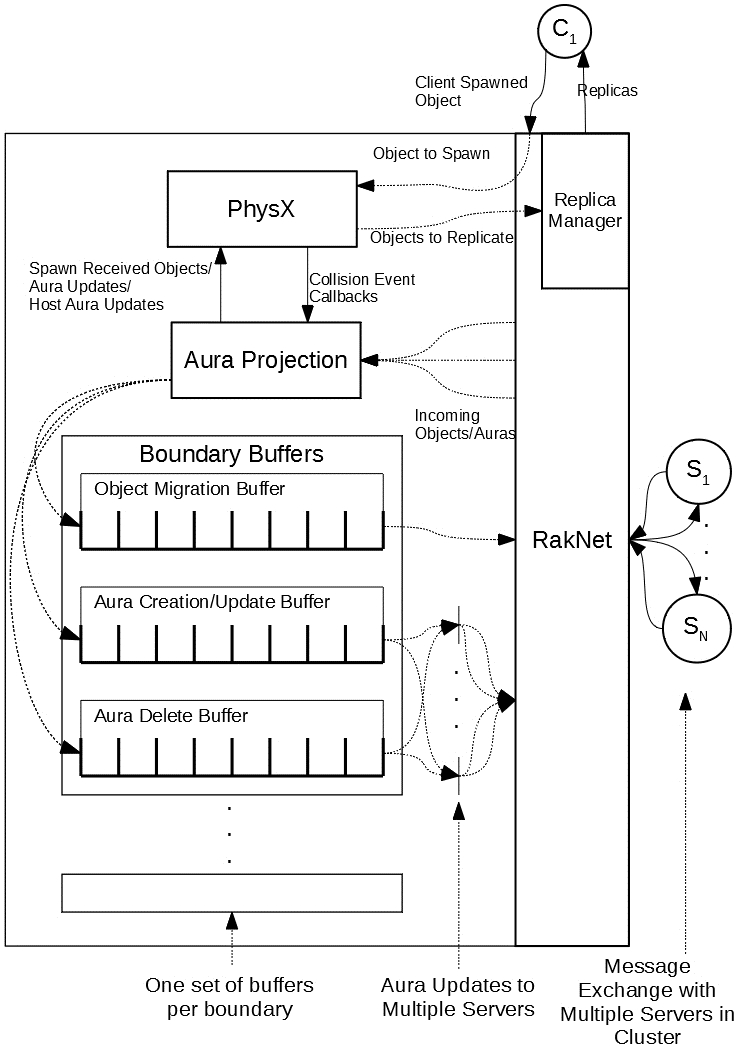
\includegraphics[width=\textwidth]{ArchitectureDiagramVertical}
	\caption{Server Architecture}
	\label{fig_stack}
\end{figure}

\section{Algorithms}
$AC$ is called when an object collides with an aura. A recursive search is performed in order to find all objects that would lie within each object's aura, preventing thrashing as discussed in \ref{Thrashing}. Once the recursive search is complete, all objects are added to the send buffer.

\renewcommand{\algorithmicforall}{\textbf{for each}}
\algnewcommand{\LeftComment}[1]{\State \(\triangleright\) #1}
\algnewcommand\And{\textbf{and}}
\algnewcommand\Or{\textbf{or}}

\begin{algorithm}
	\caption{Object Migrate - Aura Collision ($AC$)}\label{auraAlgorithm}
	\begin{algorithmic}[1]
		\Procedure{OnAuraEnter}{}	\Comment{A callback on an object}
		\LeftComment{Track visited objects to prevent infinite recursion}
		\State $\textit{visited := \{\}}$
		\LeftComment{Recursively send object with objects that would lie within each object's aura}
		\State \Call{SendWithOverlaps}{$\textit{thisObject, visited}$}
		\EndProcedure
		\State
		\Procedure{SendWithOverlaps}{$\textit{object, visited}$}
		\LeftComment{Get objects whose auras overlap this object's aura} %using a $\mathcal{O}(n)$ scene query
		\State $\textit{overlaps :=}$ \Call{GetAuraOverlaps}{$\textit{object}$} %\Comment{$\mathcal{O}(n)$ scene query}
		\State
		\ForAll{{$\textit{object} \in \textit{overlaps}$}} :
		\If {$\textit{object} \not \in \textit{visited}$}:
		\State $\textit{visited := visited + object}$
		\State \Call{SendWithOverlaps}{$\textit{object, visited}$}
		\EndIf
		\EndFor
		\State
		\State\Call{AddToSendBuffer}{object}
		\EndProcedure
	\end{algorithmic}
\end{algorithm}

$BT$ is called when an object traverses a boundary. In order to prevent `islands' forming (for example Objects H, I and J in Fig. \ref{AuraProj}), a recursive search is carried out to determine is an object is part of an island or not. If an object is found to not be part of an island, the entire cluster of objects is added to the send buffer, otherwise no action is taken.

\begin{algorithm}
	\caption{Object Migrate - Boundary Traverse ($BT$)}\label{boundaryAlgorithm}
	\begin{algorithmic}[1]	
		\LeftComment{Update called on each boundary}
		\Procedure{BoundaryUpdate}{}
		\State $\textit{checked := \{\}}$	\Comment{Used to prevent duplicate checks}
		\State
		\LeftComment{Loop over fully traversed objects from latest update}
		\ForAll{{$\textit{object} \in \textit{traversed}$}} : 
		%\If {$\textit{object.isSleeping} = \textit{false} \And \textit{object} \not \in \textit{checked}$}:
		\If {$\textit{object} \in \textit{checked}$}:
		\State $\textit{continue}$
		\EndIf
		
		\State $\textit{island := \{\}}$
		\State $\textit{isIsland := }\Call{IslandQuery}{\textit{object, island}}$
		\LeftComment{IslandQuery() returns true if object is part of an island and a list of objects in the island}
		\If {$\textit{isIsland} = \textit{true}$}:
		\State \Call{SendGroup}{$\textit{island}$}
		\EndIf
		\State $\textit{checked := checked + island}$
		\EndFor
		%		\State $\textit{visited := \{\}}$	\Comment{Track visited to prevent infinite recursion}
		%		\State \Call{SendWithOverlaps}{$\textit{thisObject, visited}$}
		\EndProcedure
		\State
		\Function{IslandQuery}{$\textit{object, visited}$}
		\State $\textit{visited := visited + object}$
		\If {$\textit{object.overlapsHostRegion = true}$}
		\State return $\textit{false}$
		\EndIf
		%\If {$\textit{object.boundaryCollisionCount = 0}$}
		%\State return $\textit{false}$
		%\EndIf
		\State
		\LeftComment{Get objects whose auras overlap this object's aura} %using a $\mathcal{O}(n)$ scene query
		\State $\textit{overlaps :=}$ \Call{GetMutalAuraOverlaps}{$\textit{object}$}
		\State
		\LeftComment{If all objects with overlapping auras are islands, then this object is an island}
		\State $\textit{isIsland := true}$
		\ForAll{{$\textit{object} \in \textit{overlaps}$}} :
		\If {$\textit{object} \not \in \textit{visited}$}:
		\State $\textit{isIsland \&= }\Call{IslandQuery}{\textit{object,visited}$}
		\EndIf
		\EndFor
		\State return $\textit{isIsland}$
		\EndFunction
		%		
		%		\Procedure{SendWithOverlaps}{$\textit{object, visited}$}
		%		\State $\textit{overlaps :=}$ \Call{GetOverlaps}{$\textit{object}$} \Comment{$\mathcal{O}(n)$ scene query}
		%		\ForAll{{$\textit{object} \in \textit{overlaps}$}} :
		%		\If {$\textit{object} \not \in \textit{visited}$}:
		%		\State $\textit{visited := visited + object}$
		%		\State \Call{SendWithOverlaps}{$\textit{object, visited}$}
		%		\EndIf
		%		\EndFor
		%		
		%		\State\Call{Send}{object}
		%		\EndProcedure
	\end{algorithmic}
\end{algorithm}

$OBC$ is called when an object collides with a boundary. The object's aura is calculated and added to the boundary's send aura buffer. A host aura is also created, to allow for the checking of mutual aura overlaps and prevent thrashing, if this is the first boundary intersection.

\begin{algorithm}
	\caption{Create Aura - Object boundary collision ($OBC$)}\label{createAuraBoundaryAlgorithm}
	\begin{algorithmic}[1]
		\LeftComment{A callback on an object, called when an object collides with a boundary}
		\Procedure{OnBoundaryEnter}{$\textit{boundary}$}
		\State \Call{AddToAuraBuffer}{$\textit{boundary, this}$}
		\State
		\LeftComment{Create `host aura' so GetMutalAuraOverlaps() will detect this object's aura}
		\If {$\textit{boundaryIntersections = 0}$}
		\State \Call{CreateHostAura}{$\textit{}$}
		\EndIf
		\State $\textit{boundaryIntersections := boundaryIntersections + 1}$
		%\State $\textit{boundariesEntered := boundariesEntered + boundary}$
		%	\State $\textit{boundary->addToOverlappingOtherObjects(m_rigidDynamic)}$
		%	\State $\textit{boundary->addBoundaryBodyToSendBuffer(this)}$
		\EndProcedure
	\end{algorithmic}
\end{algorithm}

$OBU$ is called once per frame that an object is intersecting a boundary. If the object is not `sleeping', a new aura is calculated and added to the boundary's send buffer and the host aura is updated.

The isSleeping() function returns true if an object is sleeping. From the PhysX documentation:
An object is considered `sleeping' when an actor does not move for a period of time. (The default PhysX period of time is $0.4s$ and this is the value used in our approach). Objects are `woken up' when they are touched by an awake object. 

\begin{algorithm}
	\caption{Update Aura - Object boundary update ($OBU$)}\label{objectWithAuraAlgorithm}
	\begin{algorithmic}[1]
		\LeftComment{A callback on an object, called per step per boundary the object is colliding with}
		\Procedure{onBoundaryUpdate}{$\textit{boundary}$}
		\If {$\textit{this.isSleeping = true}$}
		\State $\textit{return}$
		\EndIf
		\LeftComment{Send Aura Delta}
		\State \Call{AddToAuraBuffer}{$\textit{boundary, this}$} 
		\State \Call{UpdateHostAura}{$\textit{}$}
		%		if (!m_hasBeenSent 
		%	&& (m_app->isBoundaryOtherActor(triggerPair.triggerActor))
		%	&& !m_rigidDynamic->isSleeping()
		%	&& !m_rigidDynamic->getAngularVelocity().isZero()
		%	&& !m_rigidDynamic->getLinearVelocity().isZero()
		%	)
		%	{
		%		OrionBoundaryOther* boundary = (OrionBoundaryOther*)triggerPair.triggerActor->userData;
		%		boundary->addBoundaryBodyToSendBuffer(this);
		%	}
		%	
		%	if (m_app->isBoundaryOtherActor(triggerPair.triggerActor))
		%	{
		%		updateBoundingBox();
		%	}
		\EndProcedure
	\end{algorithmic}
\end{algorithm}

$OBE$ is called when an object is no longer intersecting a boundary. The object is added to the boundary's remove aura buffer. If the object is no longer intersecting any boundaries, the host aura is deleted.

\begin{algorithm}
	\caption{Destroy Aura - Object boundary exit ($OBE$)}\label{destroyAuraAlgorithm}
	\begin{algorithmic}[1]
		\LeftComment{A callback on an object, called when an object exits a boundary}
		\Procedure{onBoundaryExit}{$\textit{boundary}$}
		\State \Call{AddtoDeleteAuraBuffer}{$\textit{}$}
		\State
		\LeftComment{If object is no longer sending an aura, no need to keep a `host aura'}
		\State $\textit{boundaryIntersections := boundaryIntersections - 1}$
		\If {$\textit{boundaryIntersections = 0}$}
		\State \Call{DeleteHostAura}{$\textit{}$}
		\EndIf
		
		%	// If leaving boundary of other simulation, send message removing object from other boundary triggers
		%	if (!m_hasBeenSent && m_app->isBoundaryOtherActor(triggerPair.triggerActor))
		%	{
		%		OrionBoundaryOther* boundary = (OrionBoundaryOther*)triggerPair.triggerActor->userData;
		%		vector<OrionBoundaryOther*>::iterator found = find(m_boundariesWithAuras.begin(), m_boundariesWithAuras.end(), boundary);
		%		if (found != m_boundariesWithAuras.end())
		%		{
		%			boundary->addBoundaryBodyRemoveToSendBuffer(m_index);
		%			boundary->removeFromOverlappingOtherObjects(m_rigidDynamic);
		%			m_boundariesWithAuras.erase(find(m_boundariesWithAuras.begin(), m_boundariesWithAuras.end(), boundary));
		%		}
		%	}
		%	
		%	if (m_app->isBoundaryOtherActor(triggerPair.triggerActor))
		%	{
		%		m_partiallyInsideOtherCount--;
		%		PX_ASSERT(m_partiallyInsideOtherCount >= 0);
		%		if (m_partiallyInsideOtherCount == 0)
		%		{
		%			deleteBoundingBox();
		%		}
		%	}
		\EndProcedure
	\end{algorithmic}
\end{algorithm}

$BNU$ is called once per network connection between servers. It is responsible for sending and receiving object migrations and auras between servers, including the sending and receiving of auras from boundaries between other neighbouring remote servers.

\begin{algorithm}
	\caption{Boundary Network Update ($BNU$)}\label{boundaryNetworkAlgorithm}
	\begin{algorithmic}[1]
		\LeftComment{Update called once per network connection}
		\Procedure{Network Update}{}
		\LeftComment{Exchange migrations with target server}
		\State \Call{SendObjectsInBuffer}{}
		\State \Call{ReceiveObjects}{}
		\State
		\LeftComment{Send aura state updates to all neighbours}
		\ForAll{{$\textit{neighbour} \in \textit{neighbours}$}} :
		\State \Call{SendAurasInBuffer}{}
		\State \Call{SendDeleteAurasInBuffer}{}
		\State \Call{ReceiveAuras}{}
		\State \Call{ReceiveDeleteAuras}{}
		\EndFor
		%	sendRigidDynamics();
		%recvRigidDynamicUpdate();
		%
		%vector<OrionAuraExchangeBoundary*>::const_iterator it;
		%for (it = m_auraExchange.begin(); it != m_auraExchange.end(); ++it)
		%{
		%	sendBoundaryBodies(*it);
		%	sendBoundaryBodiesRemove(*it);
		%	recvBoundaryBodyUpdate(*it);
		%	recvBoundaryBodyRemoveUpdate(*it);
		%}
		\EndProcedure
	\end{algorithmic}
\end{algorithm}

\begin{figure}[hbt]
	\centering
	\resizebox{\columnwidth}{!}{
		\begin{tikzpicture}[>=stealth',shorten >=1pt,auto,node distance=2.5cm]
		\node[initial,state,accepting,align=center] (R) {$Receive$};
		\node[initial,state,accepting] (S) [below of=R] {$Inject$};
		\node[state]         (q2) [below of=S, node distance=3cm, text width=2cm, align=center] {$Intersecting$ $Boundary$};
		\node[state]         (q1) [left of=q2, node distance=4cm]  {$Host$ $Region$};
		\node[state]         (q3) [right of=q2, node distance=4cm, text width=2cm, align=center] {$Boundary$ $Traversed$};
		\node[state]         (q4) [below of=q2, node distance=4cm] {$Sent$};
		\node[state]         (q5) [right of=q4] {$Destroyed$};
		
		
		\path[->] 
		(R) edge node {} (S)
		(S) edge [bend right] node [left, text width=2cm, align=center] {No Collision} (q1)
		(S) edge node [anchor=center, text width=1.5cm, align=left] {$OBC$} (q2)
		(S) edge [bend left] node [right, text width=2cm, align=center] {Outside Owner} (q3)
		%(q1) edge [loop above] node {} (q1)
		%(q2) edge [loop left] node {} (q2)
		(q3) edge [loop below] node [above] {$BT$} (q3)
		(q1) edge node [left, text width=2cm, align=center] {$AC$} (q4)
		(q2) edge node [anchor=center, text width=2cm, align=center] {$AC$} (q4)
		(q3) edge node [anchor=center, text width=2cm, align=center] {$BT$/$AC$} (q4)
		
		(q1) edge [bend left] node [anchor=center, text width=1.5cm, align=center, above] {$OBC$} (q2)
		(q2) edge [bend left] node [anchor=center, text width=2cm, align=center, above] {$OBE$} (q1)
		(q3) edge [bend left] node [anchor=center, text width=2cm, align=center] {Owner Collision} (q2)
		(q2) edge [bend left] node [anchor=center, above, text width=2cm, align=center] {Owner Exit} (q3)
		
		(q4) edge node {} (q5)
		
		%(S)  edge [loop above] node {a} (S)
		%edge              node {a} (q1)
		%(q1) edge [bend left]  node {a} (S)
		%edge              node {b} (q2)
		%(q2) edge [loop above] node {b} (q2)
		%edge [bend left]  node {b} (q1)
		;
		\end{tikzpicture}
	}
\end{figure}

\chapter{Experiments and Results}
\section{Scalability Experiments}
This study aims to demonstrate scalability. When more servers are added, the timeliness of the simulation improves and more objects may be supported. The performance measure of interest is the maximum frame time of a server as this indicates if the simulation can be maintained when object numbers increase (keeping a low frame-time is the goal). Therefore, an injection rate is used, that spawns moving objects into the simulation as time passes.

Experiments were performed on two layouts of servers: column layout and corner layout. The column layout experiment was performed using an increasing number of servers from 1 to 10. The regions were laid out in a column configuration as shown in Fig. \ref{ColumnLayout}. Objects are injected at a constant rate, both near and far from boundaries. Injected objects are randomly selected from the following types: sphere (radius: $0.3m$), cuboid ($0.3m\mathord{\times}0.3m\mathord{\times}1.0m$) and capsule (radius: $0.3m$, height: $2m$) and start with a random velocity from the uniform distribution of: $(-10\mathord{<}x\mathord{<}10,-10\mathord{<}y\mathord{<}0,-10\mathord{<}z\mathord{<}10)m\mathord{\cdot}s^{-1}$. $50\%$ of objects are injected in a volume of $20m\mathord{\times}20m\mathord{\times}150m$ centred $12m$ away from a boundary and $15m$ above the ground plane. $50\%$ of objects are injected in the centre of a server's region in a volume of $20m\mathord{\times}20m\mathord{\times}20m$, $15m$ above the ground plane.

\definecolor{rvwvcq}{rgb}{0.08235294117647059,0.396078431372549,0.7529411764705882}
\definecolor{sim}{rgb}{0,0.2,0.5}
\begin{figure}[!t]	\begin{tikzpicture}[line cap=round,line join=round,>=triangle 45,x=1cm,y=1cm,scale=1.5]
		\clip(-2.25,0) rectangle (8.4,3.75);
	\fill[line width=0.8pt,color=rvwvcq,fill=rvwvcq,fill opacity=0.10000000149011612] (-0.02,2.5) -- (-0.02,0.5) -- (-0.22,0.5) -- (-0.22,2.5) -- cycle;
	\fill[line width=0.8pt,color=rvwvcq,fill=rvwvcq,fill opacity=0.10000000149011612] (0.22,2.5) -- (0.22,0.5) -- (0.02,0.5) -- (0.02,2.5) -- cycle;
	\fill[line width=0.8pt,color=rvwvcq,fill=rvwvcq,fill opacity=0.10000000149011612] (2.98,2.5) -- (2.98,0.5) -- (2.78,0.5) -- (2.78,2.5) -- cycle;
	\fill[line width=0.8pt,color=rvwvcq,fill=rvwvcq,fill opacity=0.10000000149011612] (3.22,2.5) -- (3.22,0.5) -- (3.022,0.5) -- (3.022,2.5) -- cycle;
	\fill[line width=0.8pt,color=rvwvcq,fill=rvwvcq,fill opacity=0.10000000149011612] (5.98,2.5) -- (5.98,0.5) -- (5.78,0.5) -- (5.78,2.5) -- cycle;
	\fill[line width=0.8pt,color=rvwvcq,fill=rvwvcq,fill opacity=0.10000000149011612] (6.222,2.5) -- (6.222,0.5) -- (6.022,0.5) -- (6.022,2.5) -- cycle;
	\fill[line width=0.8pt,color=rvwvcq,fill=rvwvcq,fill opacity=0.10000000149011612] (-1.4,1.6) -- (-1.4,1.4) -- (-1.6,1.4) -- (-1.6,1.6) -- cycle;
	\fill[line width=0.8pt,color=rvwvcq,fill=rvwvcq,fill opacity=0.10000000149011612] (1.6,1.63) -- (1.6,1.4) -- (1.4,1.4) -- (1.4,1.6) -- cycle;
	\fill[line width=0.8pt,color=rvwvcq,fill=rvwvcq,fill opacity=0.10000000149011612] (4.6,1.6) -- (4.6,1.4) -- (4.4,1.4) -- (4.4,1.6) -- cycle;
	\fill[line width=0.8pt,color=rvwvcq,fill=rvwvcq,fill opacity=0.10000000149011612] (7.6,1.6) -- (7.6,1.4) -- (7.4,1.4) -- (7.4,1.6) -- cycle;
	\fill[line width=0.8pt,color=sim,fill=sim,fill opacity=0.1] (-2.25,3) -- (-2.25,0) -- (8.25,0) -- (8.25,3) -- cycle;
	\draw [line width=0.8pt,color=rvwvcq] (-0.02,2.5)-- (-0.02,0.5);
	\draw [line width=0.8pt,color=rvwvcq] (-0.02,0.5)-- (-0.22,0.5);
	\draw [line width=0.8pt,color=rvwvcq] (-0.22,0.5)-- (-0.22,2.5);
	\draw [line width=0.8pt,color=rvwvcq] (-0.22,2.5)-- (-0.02,2.5);
	\draw [line width=0.8pt,color=rvwvcq] (0.22,2.5)-- (0.22,0.5);
	\draw [line width=0.8pt,color=rvwvcq] (0.22,0.5)-- (0.02,0.5);
	\draw [line width=0.8pt,color=rvwvcq] (0.02,0.5)-- (0.02,2.5);
	\draw [line width=0.8pt,color=rvwvcq] (0.02,2.5)-- (0.22,2.5);
	\draw (-1.5,3.5) node[anchor=center] {Server 0};
	\draw (1.5,3.5) node[anchor=center] {Server 1};
	\draw (4.5,3.5) node[anchor=center] {\textbf{...}};
	\draw (7.5,3.5) node[anchor=center] {Server N-1};
	\draw [line width=2pt] (0,0)-- (0,3);
	\draw [line width=2pt] (3,0)-- (3,3);
	\draw [line width=0.8pt,color=rvwvcq] (2.98,2.5)-- (2.98,0.5);
	\draw [line width=0.8pt,color=rvwvcq] (2.98,0.5)-- (2.78,0.5);
	\draw [line width=0.8pt,color=rvwvcq] (2.78,0.5)-- (2.78,2.5);
	\draw [line width=0.8pt,color=rvwvcq] (2.78,2.5)-- (2.98,2.5);
	\draw [line width=0.8pt,color=rvwvcq] (3.22,2.5)-- (3.22,0.5);
	\draw [line width=0.8pt,color=rvwvcq] (3.22,0.5)-- (3.022,0.5);
	\draw [line width=0.8pt,color=rvwvcq] (3.022,0.5)-- (3.022,2.5);
	\draw [line width=0.8pt,color=rvwvcq] (3.022,2.5)-- (3.22,2.5);
	\draw [line width=2pt] (6,0)-- (6,3);
	\draw [line width=0.8pt,color=rvwvcq] (5.98,2.5)-- (5.98,0.5);
	\draw [line width=0.8pt,color=rvwvcq] (5.98,0.5)-- (5.78,0.5);
	\draw [line width=0.8pt,color=rvwvcq] (5.78,0.5)-- (5.78,2.5);
	\draw [line width=0.8pt,color=rvwvcq] (5.78,2.5)-- (5.98,2.5);
	\draw [line width=0.8pt,color=rvwvcq] (6.222,2.5)-- (6.222,0.5);
	\draw [line width=0.8pt,color=rvwvcq] (6.222,0.5)-- (6.022,0.5);
	\draw [line width=0.8pt,color=rvwvcq] (6.022,0.5)-- (6.022,2.5);
	\draw [line width=0.8pt,color=rvwvcq] (6.022,2.5)-- (6.222,2.5);
	\draw [line width=0.8pt,color=rvwvcq] (-1.4,1.6)-- (-1.4,1.4);
	\draw [line width=0.8pt,color=rvwvcq] (-1.4,1.4)-- (-1.6,1.4);
	\draw [line width=0.8pt,color=rvwvcq] (-1.6,1.4)-- (-1.6,1.6);
	\draw [line width=0.8pt,color=rvwvcq] (-1.6,1.6)-- (-1.4,1.6);
	\draw [line width=0.8pt,color=rvwvcq] (1.6,1.6)-- (1.6,1.4);
	\draw [line width=0.8pt,color=rvwvcq] (1.6,1.4)-- (1.4,1.4);
	\draw [line width=0.8pt,color=rvwvcq] (1.4,1.4)-- (1.4,1.6);
	\draw [line width=0.8pt,color=rvwvcq] (1.4,1.6)-- (1.6,1.6);
	\draw [line width=0.8pt,color=rvwvcq] (4.6,1.6)-- (4.6,1.4);
	\draw [line width=0.8pt,color=rvwvcq] (4.6,1.4)-- (4.4,1.4);
	\draw [line width=0.8pt,color=rvwvcq] (4.4,1.4)-- (4.4,1.6);
	\draw [line width=0.8pt,color=rvwvcq] (4.4,1.6)-- (4.6,1.6);
	\draw [line width=0.8pt,color=rvwvcq] (7.6,1.6)-- (7.6,1.4);
	\draw [line width=0.8pt,color=rvwvcq] (7.6,1.4)-- (7.4,1.4);
	\draw [line width=0.8pt,color=rvwvcq] (7.4,1.4)-- (7.4,1.6);
	\draw [line width=0.8pt,color=rvwvcq] (7.4,1.6)-- (7.6,1.6);
	\end{tikzpicture}
\centering
\begin{tikzpicture}[line cap=round,line join=round,>=triangle 45,x=1cm,y=1cm]
		\clip(-7,0.575) rectangle (7,0.9);
\fill[line width=0.8pt,color=rvwvcq,fill=rvwvcq,fill opacity=0.1] (-2.5,0.8) -- (-2.3,0.8) -- (-2.3,0.6) -- (-2.5,0.6) -- cycle;
\draw [line width=0.8pt,color=rvwvcq] (-2.5,0.8)-- (-2.3,0.8);
\draw [line width=0.8pt,color=rvwvcq] (-2.3,0.8)-- (-2.3,0.6);
\draw [line width=0.8pt,color=rvwvcq] (-2.3,0.6)-- (-2.5,0.6);
\draw [line width=0.8pt,color=rvwvcq] (-2.5,0.6)-- (-2.5,0.8);
\draw (-2.1,0.7) node[anchor=west] {Injection Volume};

\draw [line width=2pt] (-6.5,0.7)-- (-6.3,0.7);
\draw (-6.1,0.7) node[anchor=west] {Region Boundary};
\end{tikzpicture}
\caption{Column Layout}
\label{ColumnLayout}
\end{figure}

The experiments were run for 60 seconds with an injection rate of 160 objects per second. For all experiments, a speed tolerance of $32m\mathord{\cdot}s^{-1}$ was used, which was the maximum expected speed for any object (based on maximum injection height and velocity, and gravity). The latency tolerance for these experiments was set to $2ms$ (based off measurements of latency between servers) and frame-time tolerance was set to $15ms$ (based off preliminary performance results). A time of $16ms$ was used for the physics time-step. Each experiment was repeated 50 times at various times of day to account for differing performance in cloud resources at different times. For each iteration, the maximum frame time of any server was aggregated for each $5s$ period. The mean of the aggregated maximum frame times of the iterations was then calculated and plotted.

Experiments were conducted using AWS G2.2xlarge servers located within the same geographical region. A G2.2xlarge instance uses a 2.60GHz Intel Xeon E5-2670 CPU with 16GB RAM and an NVIDIA GRID K520 (Kepler) GPU running Amazon Linux AMI 2017.09.

Fig. \ref{fig_PerCol} shows the performance of our system with rising server numbers from 1 to 10. The graph clearly shows that the addition of servers lowers the frame time throughout the experiment. This is increasingly noticeable later in the simulation when a greater number of objects are present. For higher server numbers the reduction in maximum frame time is less than for lower numbers, which is as expected as in the ideal case the workload per server would be $1/n$ of the total workload, where $n$ is the number of servers. 

From these observations it may be declared that this system is scalable in column configuration as the addition of servers results in increased performance.

\begin{figure}[!t]
	\centering
	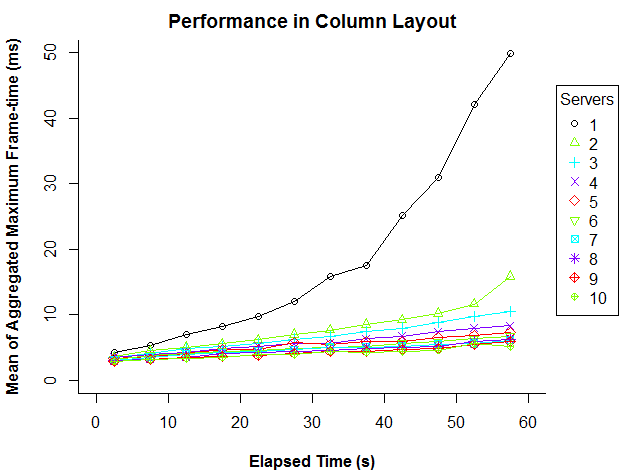
\includegraphics[width=\textwidth]{ColPerformance}
	\caption{Performance of increasing numbers of servers with an accumulating number of objects (in column layout)}
	\label{fig_PerCol}
\end{figure}

Experiments were also carried out using servers in a corner layout. The layouts of 3 and 4 servers are shown in Fig. \ref{ServerCorner}, in which the 4 server case is a 2x2 grid with a single corner intersection in the centre. The 9 server case is a 3x3 grid with 4 corner intersections. Injection rates and volume dimensions remain the same as in the column based experiments. Fig. \ref{fig_PerCor} shows the graph describing performance. The graph demonstrates that increasing the number of servers lowers the frame time. The additional processing overhead of exchanging more messages with more neighbouring servers in the 9 server experiment is outweighed by the performance gains of additional servers.

From these observations it may be declared that this system is scalable in corner configuration as the addition of servers results in increased performance.

\begin{figure}[!t]
	\begin{subfigure}{.5\textwidth}
		\begin{tikzpicture}[line cap=round,line join=round,>=triangle 45,x=1cm,y=1cm,scale=1.2]
		%	\clip(-3,-1.5) rectangle (3,3);
		\fill[line width=0.8pt,color=rvwvcq,fill=rvwvcq,fill opacity=0.10000000149011612] (-1,-0.02) -- (1,-0.02) -- (1,-0.22) -- (-1,-0.22) -- cycle;
		\fill[line width=0.8pt,color=rvwvcq,fill=rvwvcq,fill opacity=0.10000000149011612] (-0.02,2.5) -- (-0.02,0.5) -- (-0.22,0.5) -- (-0.22,2.5) -- cycle;
		\fill[line width=0.8pt,color=rvwvcq,fill=rvwvcq,fill opacity=0.10000000149011612] (0.22,2.5) -- (0.22,0.5) -- (0.02,0.5) -- (0.02,2.5) -- cycle;
		\fill[line width=0.8pt,color=rvwvcq,fill=rvwvcq,fill opacity=0.10000000149011612] (-2.5,0.22) -- (-0.5,0.22) -- (-0.5,0.02) -- (-2.5,0.02) -- cycle;
		\fill[line width=0.8pt,color=rvwvcq,fill=rvwvcq,fill opacity=0.10000000149011612] (0.5,0.22) -- (2.5,0.22) -- (2.5,0.022) -- (0.5,0.022) -- cycle;
		\fill[line width=0.8pt,color=sim,fill=sim,fill opacity=0.1] (-3,3) -- (-3,-2) -- (3,-2) -- (3,3) -- cycle;
		\draw [line width=2pt] (-3,0)-- (3,0);
		\draw [line width=2pt] (0,3)-- (0,0);
		\draw [line width=0.8pt,color=rvwvcq] (-1,-0.02)-- (1,-0.02);
		\draw [line width=0.8pt,color=rvwvcq] (1,-0.02)-- (1,-0.22);
		\draw [line width=0.8pt,color=rvwvcq] (1,-0.22)-- (-1,-0.22);
		\draw [line width=0.8pt,color=rvwvcq] (-1,-0.22)-- (-1,-0.02);
		\draw [line width=0.8pt,color=rvwvcq] (-0.02,2.5)-- (-0.02,0.5);
		\draw [line width=0.8pt,color=rvwvcq] (-0.02,0.5)-- (-0.22,0.5);
		\draw [line width=0.8pt,color=rvwvcq] (-0.22,0.5)-- (-0.22,2.5);
		\draw [line width=0.8pt,color=rvwvcq] (-0.22,2.5)-- (-0.02,2.5);
		\draw [line width=0.8pt,color=rvwvcq] (0.22,2.5)-- (0.22,0.5);
		\draw [line width=0.8pt,color=rvwvcq] (0.22,0.5)-- (0.02,0.5);
		\draw [line width=0.8pt,color=rvwvcq] (0.02,0.5)-- (0.02,2.5);
		\draw [line width=0.8pt,color=rvwvcq] (0.02,2.5)-- (0.22,2.5);
		\draw (-1.5,2.5) node[anchor=center] {Server 0};
		\draw (1.5,2.5) node[anchor=center] {Server 1};
		\draw (0,-1) node[anchor=center] {Server 2};
		\draw [line width=0.8pt,color=rvwvcq] (-2.5,0.22)-- (-0.5,0.22);
		\draw [line width=0.8pt,color=rvwvcq] (-0.5,0.22)-- (-0.5,0.02);
		\draw [line width=0.8pt,color=rvwvcq] (-0.5,0.02)-- (-2.5,0.02);
		\draw [line width=0.8pt,color=rvwvcq] (-2.5,0.02)-- (-2.5,0.22);
		\draw [line width=0.8pt,color=rvwvcq] (0.5,0.22)-- (2.5,0.22);
		\draw [line width=0.8pt,color=rvwvcq] (2.5,0.22)-- (2.5,0.022);
		\draw [line width=0.8pt,color=rvwvcq] (2.5,0.022)-- (0.5,0.022);
		\draw [line width=0.8pt,color=rvwvcq] (0.5,0.022)-- (0.5,0.22);
		\draw [line width=0.8pt,color=rvwvcq] (-1.4,1.6)-- (-1.4,1.4);
		\draw [line width=0.8pt,color=rvwvcq] (-1.4,1.4)-- (-1.6,1.4);
		\draw [line width=0.8pt,color=rvwvcq] (-1.6,1.4)-- (-1.6,1.6);
		\draw [line width=0.8pt,color=rvwvcq] (-1.6,1.6)-- (-1.4,1.6);
		\draw [line width=0.8pt,color=rvwvcq] (1.6,1.6)-- (1.6,1.4);
		\draw [line width=0.8pt,color=rvwvcq] (1.6,1.4)-- (1.4,1.4);
		\draw [line width=0.8pt,color=rvwvcq] (1.4,1.4)-- (1.4,1.6);
		\draw [line width=0.8pt,color=rvwvcq] (1.4,1.6)-- (1.6,1.6);
		
		\draw [line width=0.8pt,color=rvwvcq] (0.1,-1.6)-- (0.1,-1.4);
		\draw [line width=0.8pt,color=rvwvcq] (0.1,-1.4)-- (-0.1,-1.4);
		\draw [line width=0.8pt,color=rvwvcq] (-0.1,-1.4)-- (-0.1,-1.6);
		\draw [line width=0.8pt,color=rvwvcq] (-0.1,-1.6)-- (0.1,-1.6);
		\end{tikzpicture}
		\centering
		\begin{tikzpicture}[line cap=round,line join=round,>=triangle 45,x=1cm,y=1cm]
		%		\clip(-3.661612836111066,-0.55) rectangle (6.690195527240868,1.05);
		\fill[line width=0.8pt,color=rvwvcq,fill=rvwvcq,fill opacity=0.10000000149011612] (-2.5,0.22) -- (-2.3,0.22) -- (-2.3,0.02) -- (-2.5,0.02) -- cycle;
		\draw [line width=0.8pt,color=rvwvcq] (-2.5,0.22)-- (-2.3,0.22);
		\draw [line width=0.8pt,color=rvwvcq] (-2.3,0.22)-- (-2.3,0.02);
		\draw [line width=0.8pt,color=rvwvcq] (-2.3,0.02)-- (-2.5,0.02);
		\draw [line width=0.8pt,color=rvwvcq] (-2.5,0.02)-- (-2.5,0.22);
		\draw [line width=2pt] (-2.5,0.5)-- (-2.3,0.5);
		\draw (-2.1,0.5) node[anchor=west] {Region Boundary};
		\draw (-2.1,0.1) node[anchor=west] {Injection Volume};
		\end{tikzpicture}
		\caption{3 Server Corner Layout}
		\label{3ServerCorner}
	\end{subfigure}%
	\begin{subfigure}{.5\textwidth}
		\begin{tikzpicture}[line cap=round,line join=round,>=triangle 45,x=1cm,y=1cm,scale=1.2]
		%	\clip(-3,-3) rectangle (3,3);
		\fill[line width=0.8pt,color=rvwvcq,fill=rvwvcq,fill opacity=0.10000000149011612] (0.5,-0.02) -- (2.5,-0.02) -- (2.5,-0.22) -- (0.5,-0.22) -- cycle;
		\fill[line width=0.8pt,color=rvwvcq,fill=rvwvcq,fill opacity=0.10000000149011612] (-0.02,2.5) -- (-0.02,0.5) -- (-0.22,0.5) -- (-0.22,2.5) -- cycle;
		\fill[line width=0.8pt,color=rvwvcq,fill=rvwvcq,fill opacity=0.10000000149011612] (0.22,2.5) -- (0.22,0.5) -- (0.02,0.5) -- (0.02,2.5) -- cycle;
		\fill[line width=0.8pt,color=rvwvcq,fill=rvwvcq,fill opacity=0.10000000149011612] (-2.5,0.22) -- (-0.5,0.22) -- (-0.5,0.02) -- (-2.5,0.02) -- cycle;
		\fill[line width=0.8pt,color=rvwvcq,fill=rvwvcq,fill opacity=0.10000000149011612] (0.5,0.22) -- (2.5,0.22) -- (2.5,0.022) -- (0.5,0.022) -- cycle;
		\fill[line width=0.8pt,color=rvwvcq,fill=rvwvcq,fill opacity=0.10000000149011612] (-0.02,-0.5) -- (-0.02,-2.5) -- (-0.22,-2.5) -- (-0.22,-0.5) -- cycle;
		\fill[line width=0.8pt,color=rvwvcq,fill=rvwvcq,fill opacity=0.10000000149011612] (0.22,-0.5) -- (0.22,-2.5) -- (0.02,-2.5) -- (0.02,-0.5) -- cycle;
		\fill[line width=0.8pt,color=rvwvcq,fill=rvwvcq,fill opacity=0.10000000149011612] (-2.5,-0.022) -- (-0.5,-0.022) -- (-0.5,-0.22) -- (-2.5,-0.22) -- cycle;
		\fill[line width=0.8pt,color=sim,fill=sim,fill opacity=0.1] (-3,3) -- (-3,-3) -- (3,-3) -- (3,3) -- cycle;
		\draw [line width=2pt] (-3,0)-- (3,0);
		\draw [line width=2pt] (0,3)-- (0,0);
		\draw [line width=0.8pt,color=rvwvcq] (0.5,-0.02)-- (2.5,-0.02);
		\draw [line width=0.8pt,color=rvwvcq] (2.5,-0.02)-- (2.5,-0.22);
		\draw [line width=0.8pt,color=rvwvcq] (2.5,-0.22)-- (0.5,-0.22);
		\draw [line width=0.8pt,color=rvwvcq] (0.5,-0.22)-- (0.5,-0.02);
		\draw [line width=0.8pt,color=rvwvcq] (-0.02,2.5)-- (-0.02,0.5);
		\draw [line width=0.8pt,color=rvwvcq] (-0.02,0.5)-- (-0.22,0.5);
		\draw [line width=0.8pt,color=rvwvcq] (-0.22,0.5)-- (-0.22,2.5);
		\draw [line width=0.8pt,color=rvwvcq] (-0.22,2.5)-- (-0.02,2.5);
		\draw [line width=0.8pt,color=rvwvcq] (0.22,2.5)-- (0.22,0.5);
		\draw [line width=0.8pt,color=rvwvcq] (0.22,0.5)-- (0.02,0.5);
		\draw [line width=0.8pt,color=rvwvcq] (0.02,0.5)-- (0.02,2.5);
		\draw [line width=0.8pt,color=rvwvcq] (0.02,2.5)-- (0.22,2.5);
		\draw (-1.5,2.5) node[anchor=center] {Server 0};
		\draw (1.5,2.5) node[anchor=center] {Server 1};
		\draw (-1.5,-2.5) node[anchor=center] {Server 2};
		\draw (1.5,-2.5) node[anchor=center] {Server 3};
		\draw [line width=0.8pt,color=rvwvcq] (-2.5,0.22)-- (-0.5,0.22);
		\draw [line width=0.8pt,color=rvwvcq] (-0.5,0.22)-- (-0.5,0.02);
		\draw [line width=0.8pt,color=rvwvcq] (-0.5,0.02)-- (-2.5,0.02);
		\draw [line width=0.8pt,color=rvwvcq] (-2.5,0.02)-- (-2.5,0.22);
		\draw [line width=0.8pt,color=rvwvcq] (0.5,0.22)-- (2.5,0.22);
		\draw [line width=0.8pt,color=rvwvcq] (2.5,0.22)-- (2.5,0.022);
		\draw [line width=0.8pt,color=rvwvcq] (2.5,0.022)-- (0.5,0.022);
		\draw [line width=0.8pt,color=rvwvcq] (0.5,0.022)-- (0.5,0.22);
		\draw [line width=0.8pt,color=rvwvcq] (-0.02,-0.5)-- (-0.02,-2.5);
		\draw [line width=0.8pt,color=rvwvcq] (-0.02,-2.5)-- (-0.22,-2.5);
		\draw [line width=0.8pt,color=rvwvcq] (-0.22,-2.5)-- (-0.22,-0.5);
		\draw [line width=0.8pt,color=rvwvcq] (-0.22,-0.5)-- (-0.02,-0.5);
		\draw [line width=0.8pt,color=rvwvcq] (0.22,-0.5)-- (0.22,-2.5);
		\draw [line width=0.8pt,color=rvwvcq] (0.22,-2.5)-- (0.02,-2.5);
		\draw [line width=0.8pt,color=rvwvcq] (0.02,-2.5)-- (0.02,-0.5);
		\draw [line width=0.8pt,color=rvwvcq] (0.02,-0.5)-- (0.22,-0.5);
		\draw [line width=2pt] (0,0)-- (0,-3);
		\draw [line width=0.8pt,color=rvwvcq] (-2.5,-0.022)-- (-0.5,-0.022);
		\draw [line width=0.8pt,color=rvwvcq] (-0.5,-0.022)-- (-0.5,-0.22);
		\draw [line width=0.8pt,color=rvwvcq] (-0.5,-0.22)-- (-2.5,-0.22);
		\draw [line width=0.8pt,color=rvwvcq] (-2.5,-0.22)-- (-2.5,-0.022);
		\draw [line width=0.8pt,color=rvwvcq] (-1.4,1.6)-- (-1.4,1.4);
		\draw [line width=0.8pt,color=rvwvcq] (-1.4,1.4)-- (-1.6,1.4);
		\draw [line width=0.8pt,color=rvwvcq] (-1.6,1.4)-- (-1.6,1.6);
		\draw [line width=0.8pt,color=rvwvcq] (-1.6,1.6)-- (-1.4,1.6);
		\draw [line width=0.8pt,color=rvwvcq] (1.6,1.6)-- (1.6,1.4);
		\draw [line width=0.8pt,color=rvwvcq] (1.6,1.4)-- (1.4,1.4);
		\draw [line width=0.8pt,color=rvwvcq] (1.4,1.4)-- (1.4,1.6);
		\draw [line width=0.8pt,color=rvwvcq] (1.4,1.6)-- (1.6,1.6);
		
		\draw [line width=0.8pt,color=rvwvcq] (-1.4,-1.6)-- (-1.4,-1.4);
		\draw [line width=0.8pt,color=rvwvcq] (-1.4,-1.4)-- (-1.6,-1.4);
		\draw [line width=0.8pt,color=rvwvcq] (-1.6,-1.4)-- (-1.6,-1.6);
		\draw [line width=0.8pt,color=rvwvcq] (-1.6,-1.6)-- (-1.4,-1.6);
		\draw [line width=0.8pt,color=rvwvcq] (1.6,-1.6)-- (1.6,-1.4);
		\draw [line width=0.8pt,color=rvwvcq] (1.6,-1.4)-- (1.4,-1.4);
		\draw [line width=0.8pt,color=rvwvcq] (1.4,-1.4)-- (1.4,-1.6);
		\draw [line width=0.8pt,color=rvwvcq] (1.4,-1.6)-- (1.6,-1.6);
		\end{tikzpicture}
		\centering
		\caption{4 Server Corner Layout}
		\label{4ServerCorner}
	\end{subfigure}
\caption{Corner Layouts}
\label{ServerCorner}
\end{figure}

\begin{figure}[!t]
	\centering
	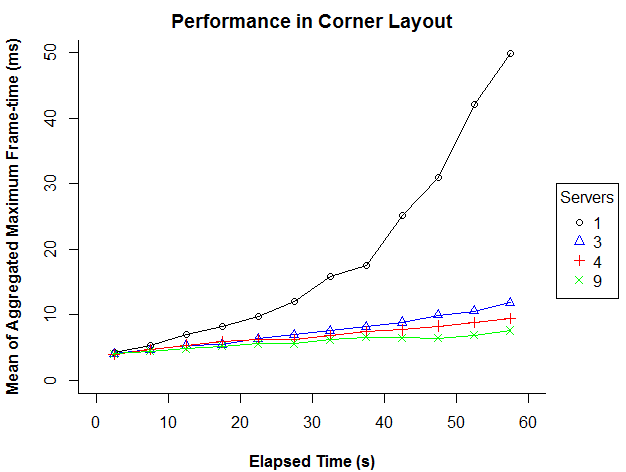
\includegraphics[width=\textwidth]{CorPerformance}
	\caption{Performance of increasing numbers of servers with an accumulating number of objects (in corner layout)}
	\label{fig_PerCor}
\end{figure}

\section{Collision Correctness Experiments}
In the following section we explore the correctness of collisions between objects, i.e. do objects have the same collision behaviour in a AP as they do in a centralised system. We are concerned with objects that are migrating and/or interacting with an object that has recently migrated.
We will now explain how a naive system can lead to erroneous collision behaviour and AP can lead to erroneous collision behaviour if speed, frame-time or latency go above the user-defined tolerances.

Erroneous collisions fall into two categories:
\begin{itemize}
	\item Missed collisions, collisions that should have taken place but were not detected by the physics engine e.g. Bullet through paper problem.
	\item Late collisions, collisions that were detected later than they should have been and result in not only different collision results, but also unstable collision response.
\end{itemize} 

%TODO: Expand on late collisions producing different results?

To understand how late collisions lead to unstable collision response, we must first understand how in real-time collision detection works. In real-time physics engines, objects move in descrete steps, as a result of this, when two objects collide, they overlap each other i.e. penetrate. The collision is resolved by calculating the forces resulting from the collision and moving the objects so they no longer overlap (in PhysX if penetration is high, the latter may be done over several physics time-steps). If the penetration is high, such as in the case of a late collision response or if two objects are moving at high speed towards one another, the collision response can no longer guarantee stable results.

It is possible to detect late collisions between objects. Given the relative speed of the two objects and the physics time-step, it possible to calculate the maximum expected penetration distance. If a collision is detected and it is above this value, it means it is a late collision.

Maximum penetration for a given speed occurs when two objects travelling directly towards each other have, in the final time-step before colliding the two objects have no distance between them, but are not overlapping, so not colliding. The next physics time-step, the collision will be detected and will have the maximum penetration possible for that relative speed. Re-arranging s=d/t, to d=s.t and substituting the physics time-step for t, gives us the maximum distance (penetration) for a relative speed, and we are able to plot the maximum expected penetration line.

%In real-time physics, speed of calculation is favoured over accuracy of collision response, as a result of this 

%, this is known as the collision response (in real-time physics, speed of calculation is favoured over accuracy of collision response). High collision penetration e.g. if two objects are moving quickly towards one another, can lead to unstable collision response, which is undesirable.

%TODO: cite that deep penetration is bad

Experiments were carried out where collision results were recorded and used to detect missed and late collisions of objects. The experiment scenario used only two objects, meaning if there was a missed collision there would be no collision output. The two objects start the scenario with a specified velocity (drag and gravity are disabled), the direction being directly towards the other object and the two objects were given the same speed, which is varied throughout the experiment. Spheres were used, so rotational effects don't need to be accounted for.

A control experiment on a centralised system was performed, in which the scenario was repeated multiple times. The purpose of this experiment was to confirm the predicted maximum expected penetration. Fig. \ref{fig_ErrorCentral} shows the penetration of objects with increasing speed in a centralised simulation and demonstrates that penetration is never greater than the maximum expected penetration.

% TODO: Add number of collisions and number of missed collisions
\begin{figure}[!t]
	\centering
	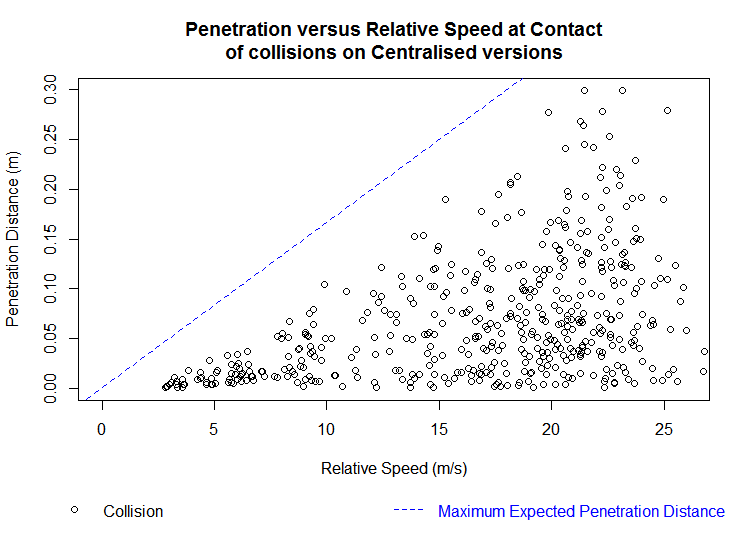
\includegraphics[width=\textwidth]{errorGraphCentral}
	\caption{Penetration of objects with increasing speed and maximum expected penetration}
	\label{fig_ErrorCentral}
\end{figure}

AP can only lead to late or missed collisions when at least one object involved in the collision has just migrated (received since the last physics time-step). This is because non-migrating objects behave the same as objects in a centralised solution. In order to test this case, the same scenario as the control was used with two servers. The two spheres were given starting positions so the two would collide at a point on the boundary between servers, thus creating the most likely situation for objects collide with each other in their first time-step after being migrated. The purpose of this experiment is to demonstrate that collisions in AP are always correct if the respective values remain within their tolerances.
Only objects that have just migrated are considered in the experiment results. The two servers use the same tolerances used in the performance experiments, including a maximum speed tolerance of $32m\mathord{\cdot}s^{-1}$.

%TODO: Graph for 2-server collisions. Will need set values with tolerances to max and vary them one at a time.

%TODO: Missed collisions (and number of, mean and max error)

\section{Communication Correctness Experiments}
%Will look for missing/duplicate objects auras. Dangling auras

\section{Case Study: Suspension Bridge}

\chapter{Conclusions and Future Work}
An approach to networked real-time physics simulations that is scalable and alleviates the processing limitation of a single server has been presented. Only open-source software has been used in our approach and our algorithm has been developed in a way that is agnostic to any specific application technology.

Our experiments establish that the approach is scalable, as demonstrated by the addition of servers improving the performance of the system when simulating an increasingly large number of objects. This study has demonstrated that a standard real-time physics engine (in this case, PhysX) may be incorporated into our scalable real-time physics system and achieve performance that is acceptable for real-time distributed simulations such as networked games.

Our continuing work will be to carry out experiments to determine the effects that increasing latency and packet loss, and varying user defined latency and speed tolerances, have on the scalability and stability of our approach. This will provide data, which may inform a dynamically adapting messaging layer that may manage cloud resources more efficiently depending on the distribution of object interaction within a simulated world. 

We are currently seeking to extend our approach to support large jointed objects that could span multiple servers. For example, a suspension bridge could be modelled in fine detail using multiple servers. This requires our approach to be extended to ensure some jointed elements may span section boundaries to connect independent objects on different servers. 

Future work will enable boundaries between regions to evolve dynamically allowing load-balancing to occur, further lowering the maximum frame time across servers. In addition to load-balancing, dynamic boundaries can routinely repartition the regions between servers to avoid or reduce the number of objects interacting over region boundaries. This will reduce both network and processing overhead by avoiding the need for auras and migrations to be exchanged between servers, further improving the performance and scalability of our approach.
